\chapter{Aplicação}\label{cap:aplicacao}

O objetivo da aplicação como descrito na seção \ref{sec:objetivos} do capítulo \ref{cap:introducao} é realizar a segmentação de imagens por meio de um aplicativo móvel na plataforma Android.
O processo de segmentação é realizado pelo algoritmo de segmentação por técnica baseada em \textit{watershed}, descrito no capítulo \ref{cap:algoritmo}, e a imagem segmentada resultante é apresentada na tela do aplicativo.

\section{Aquisição da imagem}\label{sec:aquisicao_aplicacao}

A aquisição da imagem pode ser feita de duas maneiras diferentes: 

% \section{Aquisição da imagem}
\begin{itemize}
    \item Por meio do acesso à galeria de imagens do dispositivo; e
    \item Por meio da captura de uma imagem através da câmera do dispositivo.
\end{itemize}

% Figura 
  \begin{figure}[!htb]
       \begin{center}  
          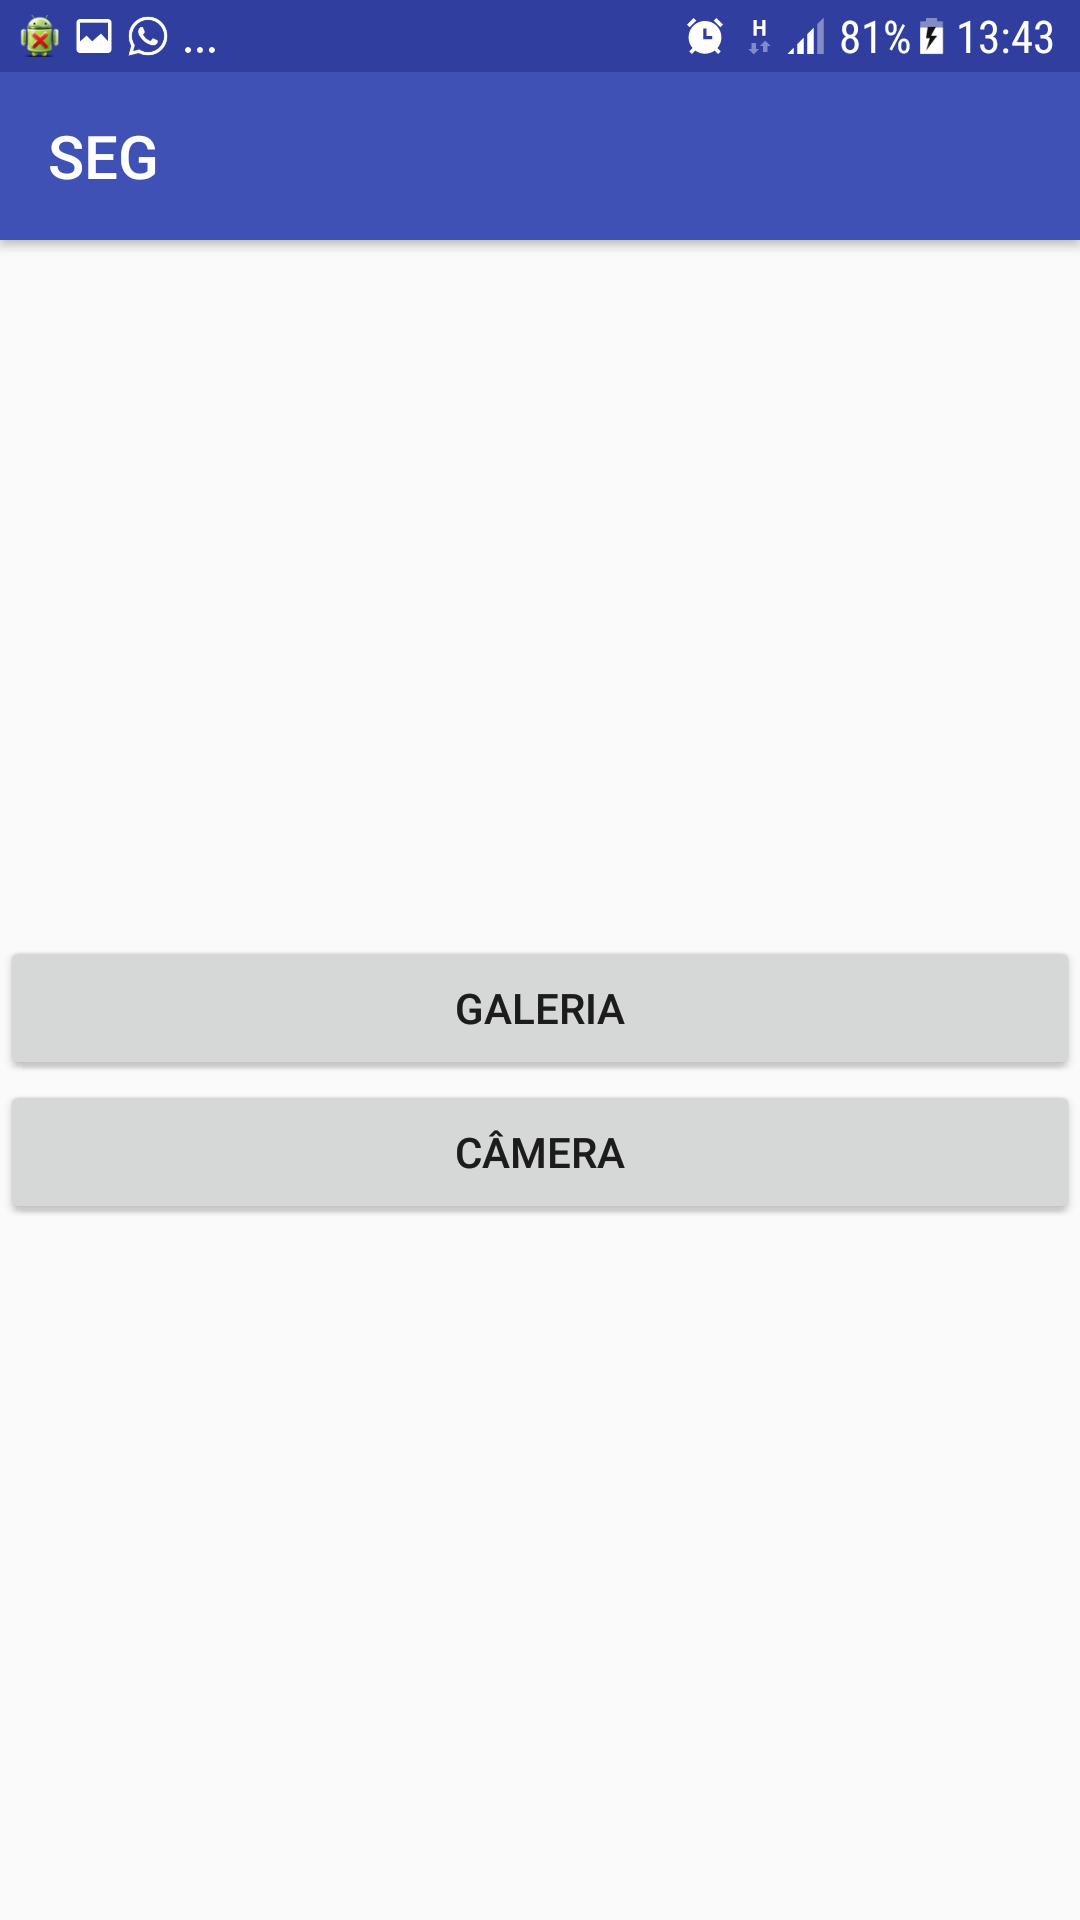
\includegraphics[width=0.3\columnwidth]{img/telainicial_app.png}
           \caption{\label{fig:telainicial_app}Tela Inicial do aplicativo.}
           % \vspace{2.0em}
       \end{center}
   \end{figure}

\subsection{Galeria de imagens}

Para escolher uma imagem a ser segmentada, deve-se clicar no botão "GALERIA" que levará a uma tela com uma imagem modelo já pré-definida e com três botões. Basta clicar no botão "LOAD" para acessar as imagens existentes no dispositivo e, depois, clicar sobre a imagem desejada a fim de carregá-la na tela.
A imagem escolhida será apresentada na tela, substituindo a imagem anterior.
% Figura 
\begin{figure}[!htb]
 \centering
 \def\baselinestretch{1}\small\normalsize
 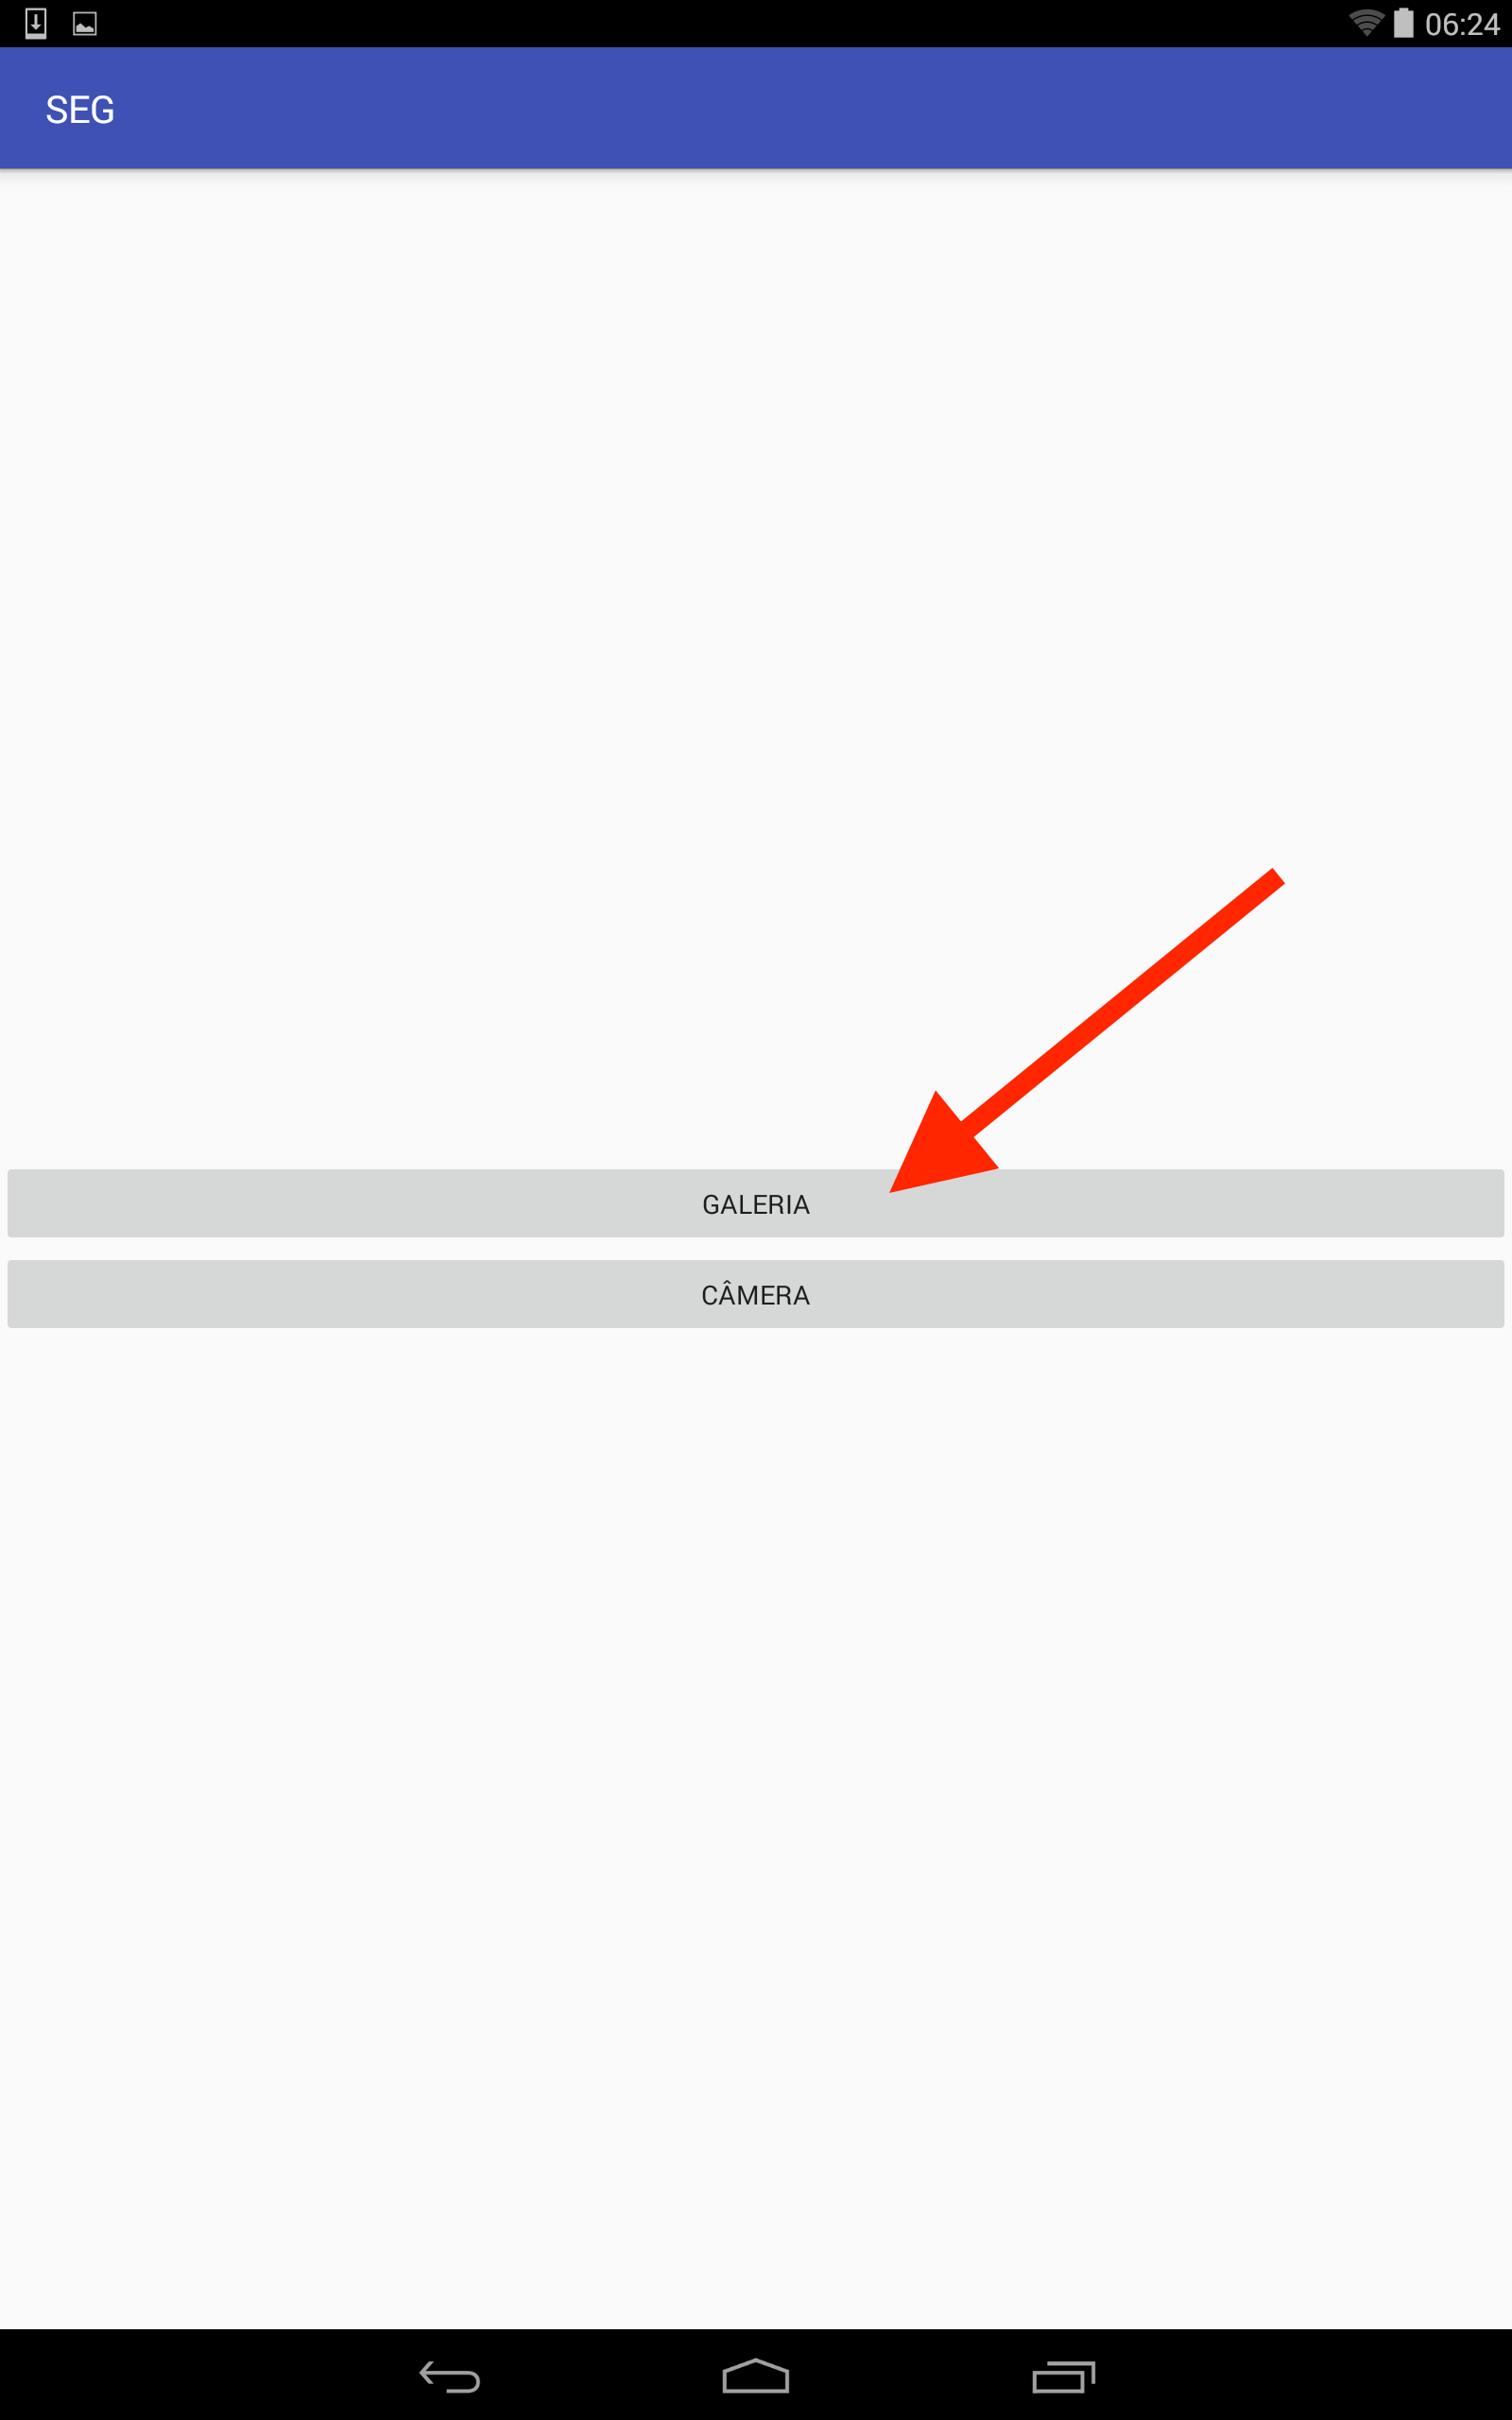
\includegraphics[width=0.4\textwidth]{img/galeria_app_n1.png}\qquad
 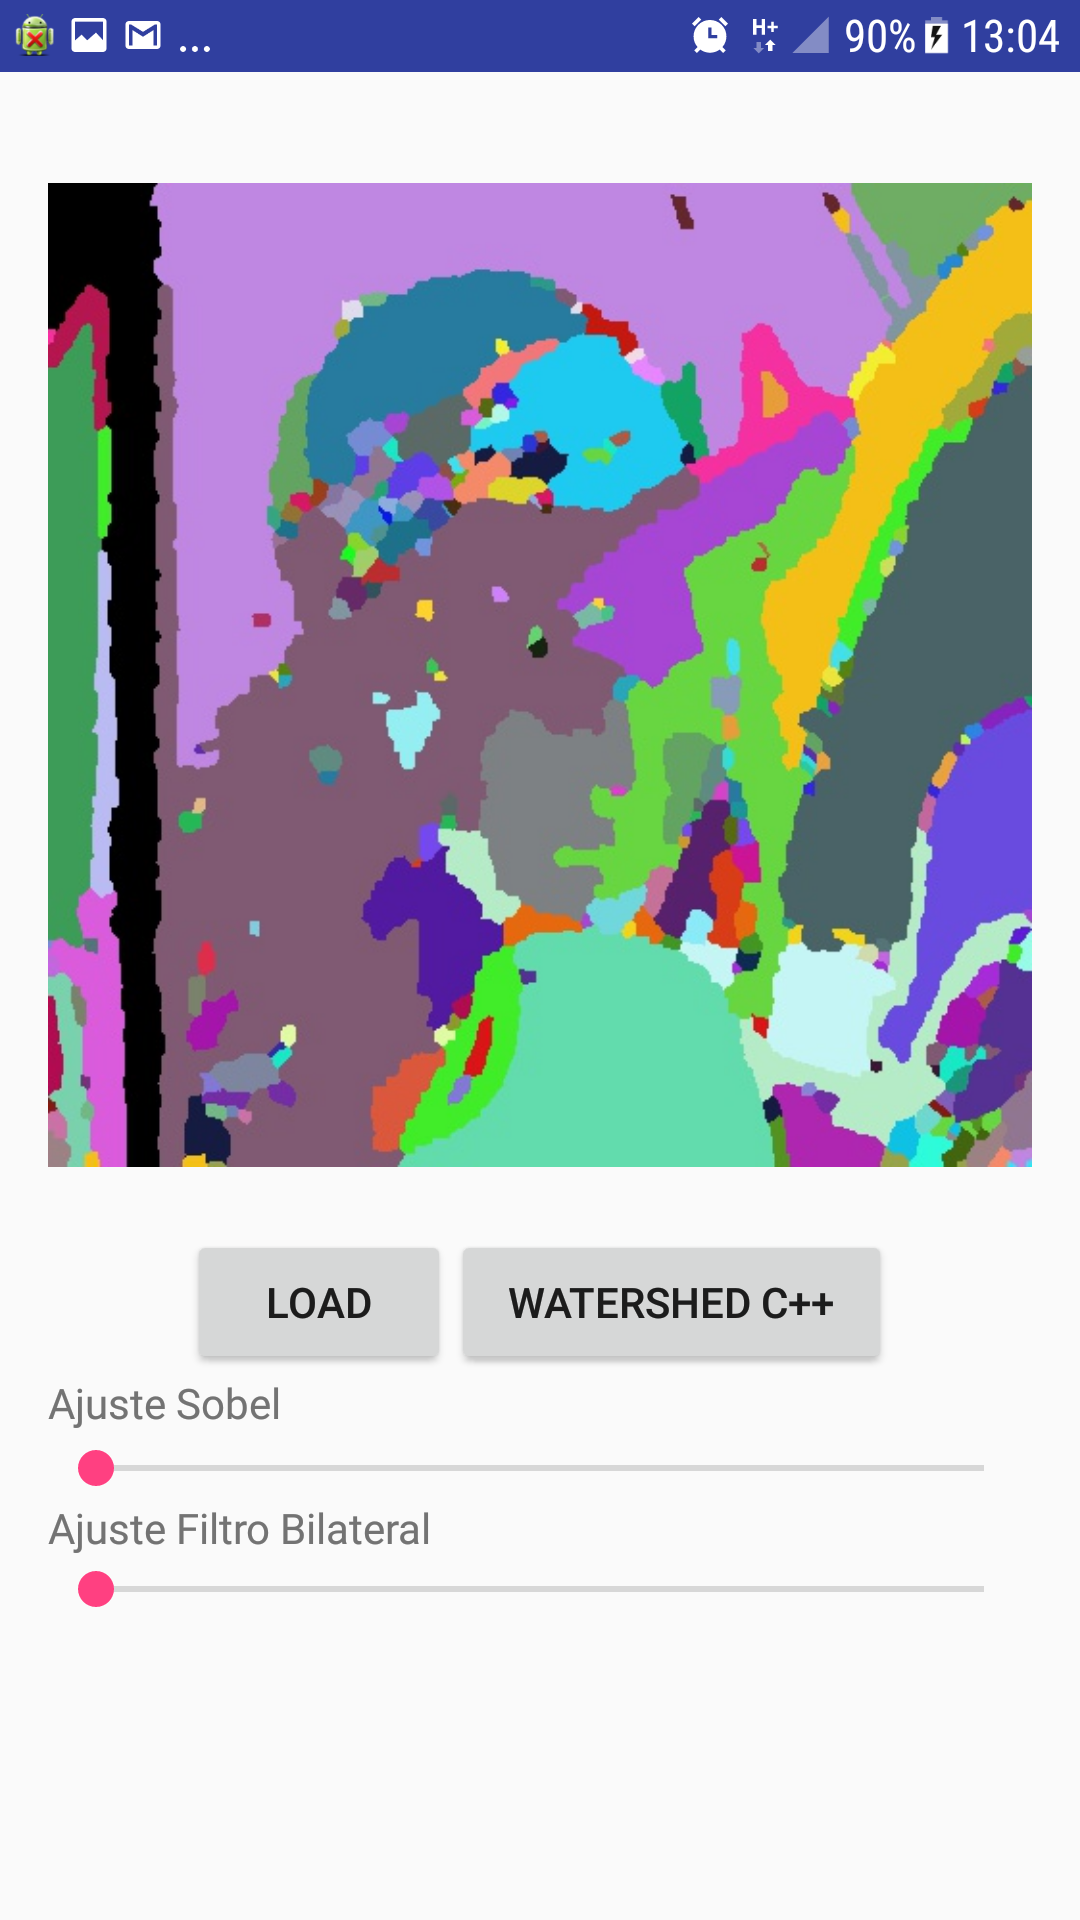
\includegraphics[width=0.4\textwidth]{img/galeria_app_n2.png} 
 \caption{\label{fig:galeria_app_p1}Sequência de atividades para aquisição da imagem por meio da galeria de imagens.}
 %\vspace{2.0em}
\end{figure}
% Figura 
\begin{figure}[!htb]
 \centering
 \def\baselinestretch{1}\small\normalsize
 \includegraphics[width=0.4\textwidth]{img/galeria_app_n3.png}\qquad
 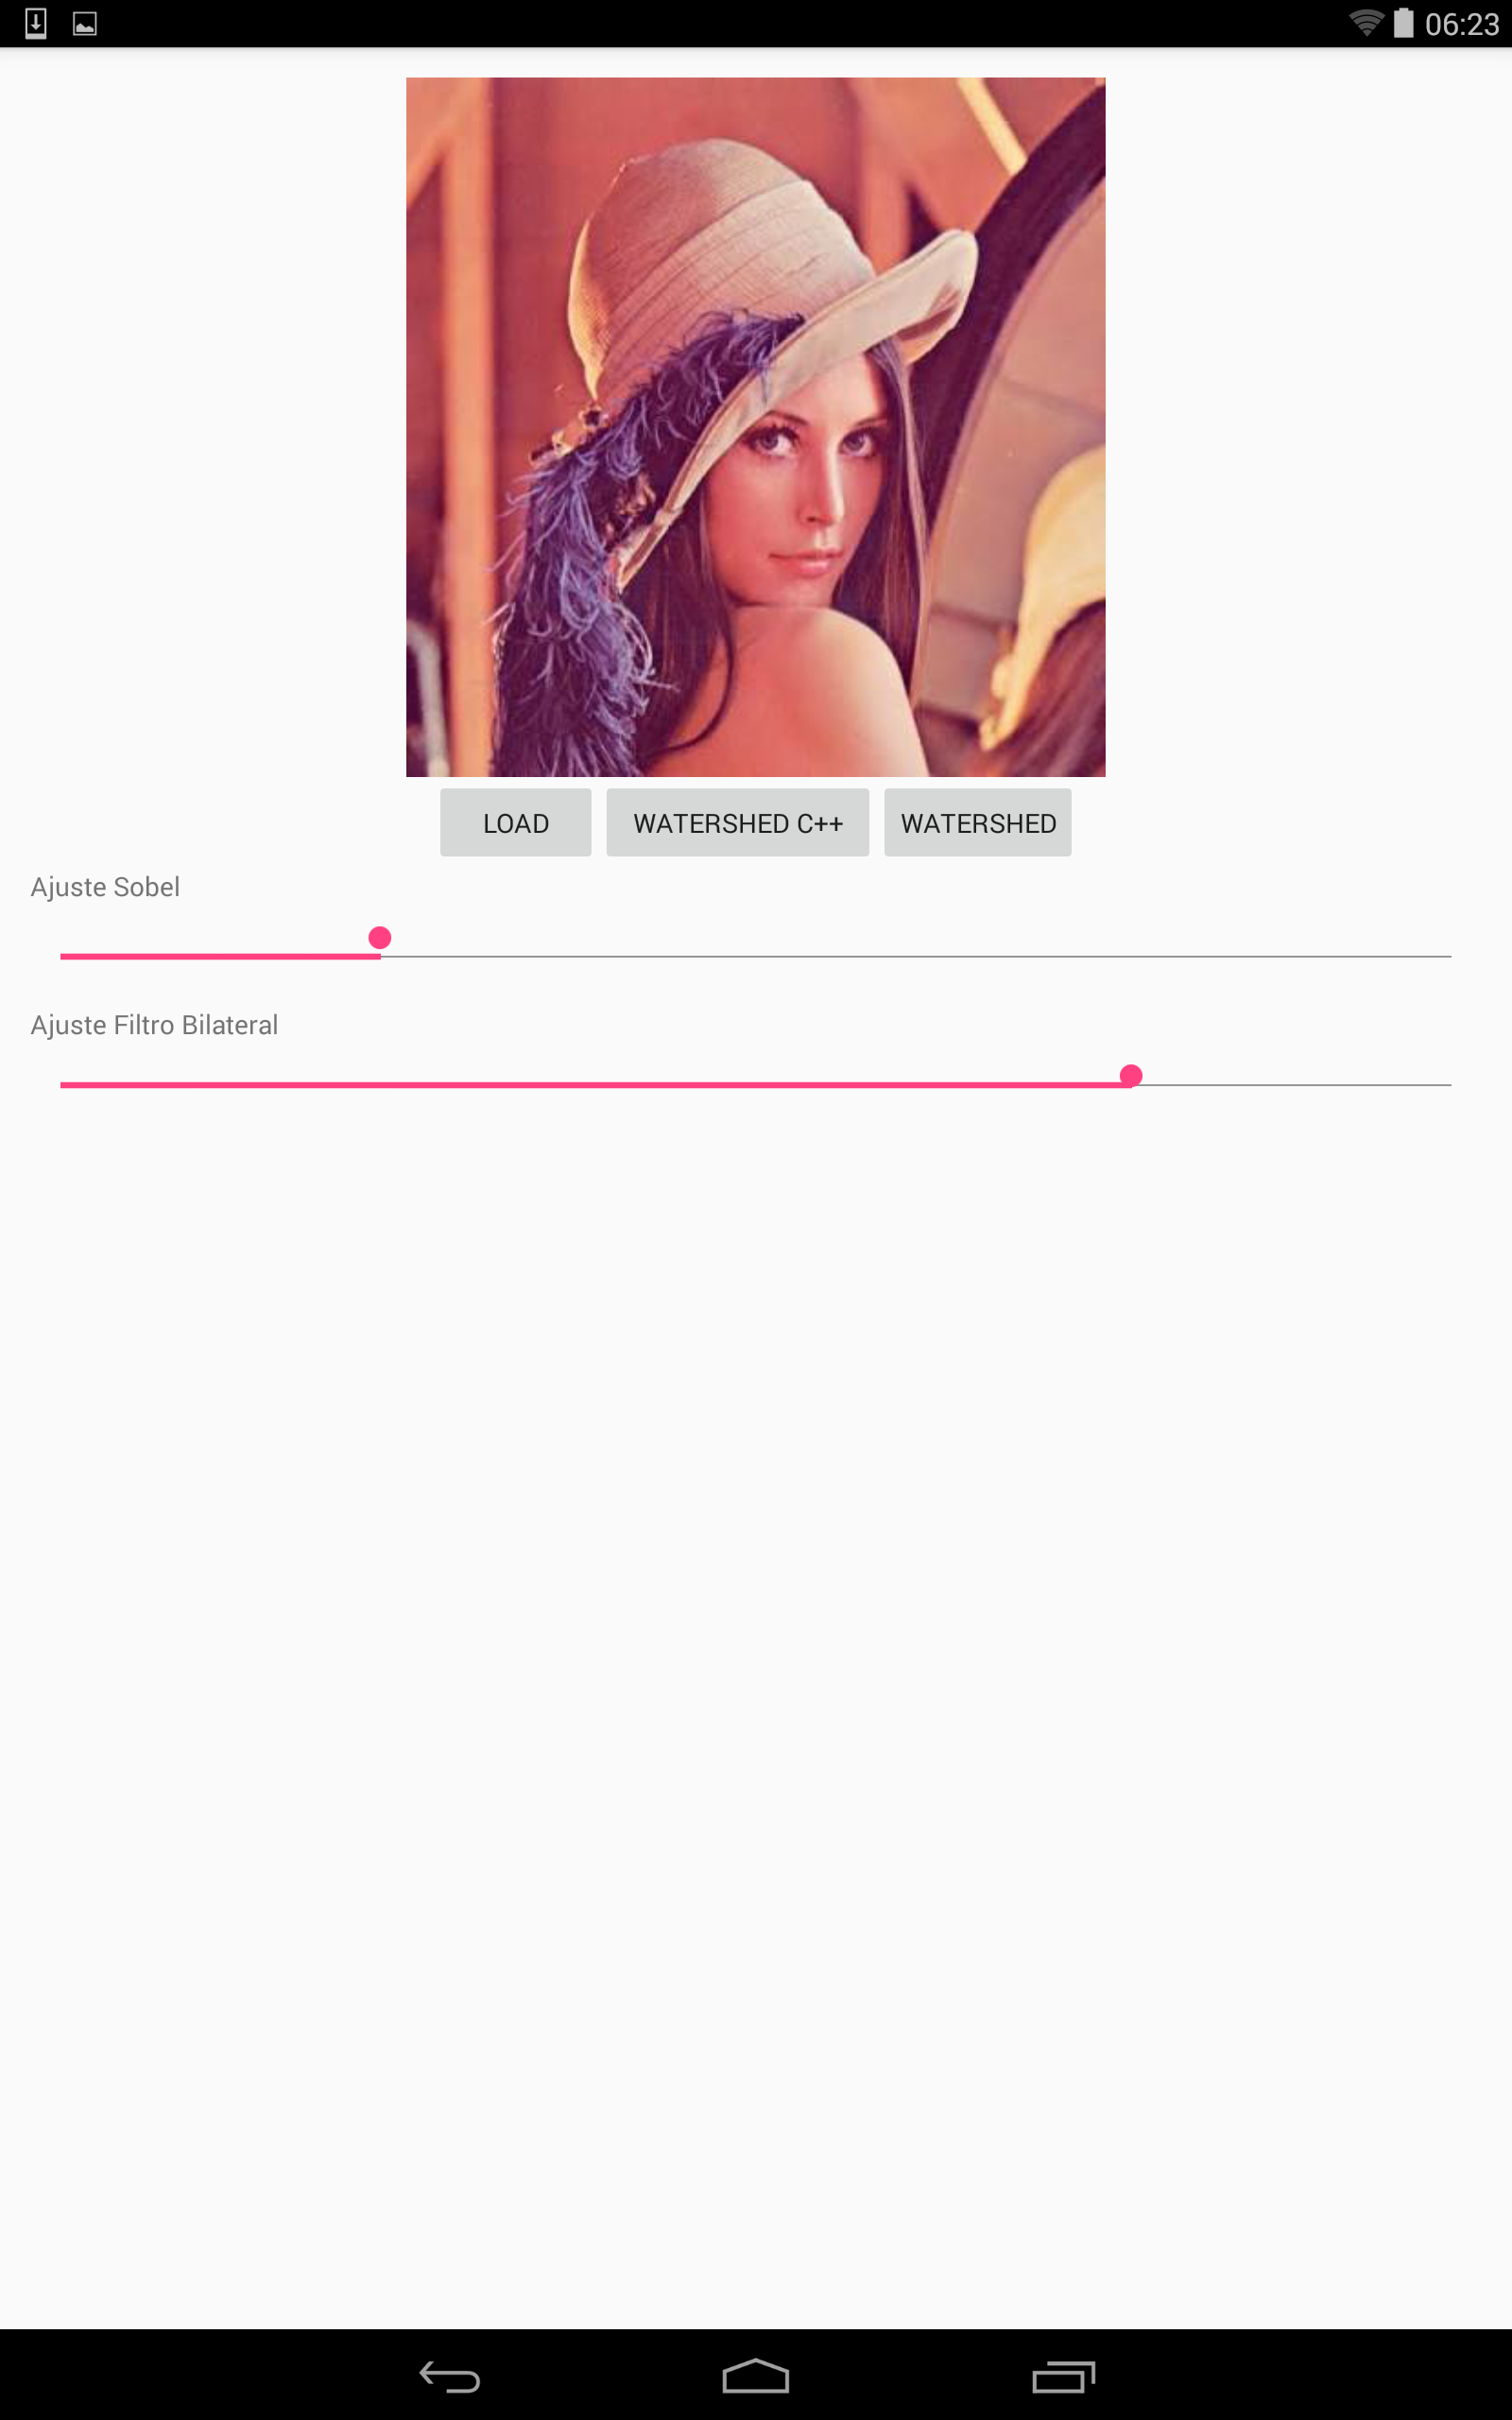
\includegraphics[width=0.4\textwidth]{img/galeria_app_n4.png} 
 \caption{\label{fig:galeria_app_p2}Sequência de atividades para aquisição da imagem por meio da galeria de imagens.}
 %\vspace{2.0em}
\end{figure}
\clearpage
 
\subsection{Câmera}

Uma nova imagem pode ser adquirida a qualquer momento para ser utilizada na segmentação por meio do acesso à câmera do dispositivo. Para acessar a câmera, basta clicar no botão "CÂMERA" apresentado na tela inicial da aplicação.
Com a câmera funcionando, pode-se aplicar diversos procedimentos de pré-processamento nas imagens em tempo real:

% \section{Procedimentos de pré-processamento}
\begin{itemize}
    \item Conversão para Cinza;
    \item Operador Sobel;
    \item Filtro Biltateral;
    \item Operação Morfológica;
    \item SIFT;
\end{itemize}
% Figura 
  \begin{figure}[!htb]
       \begin{center}  
          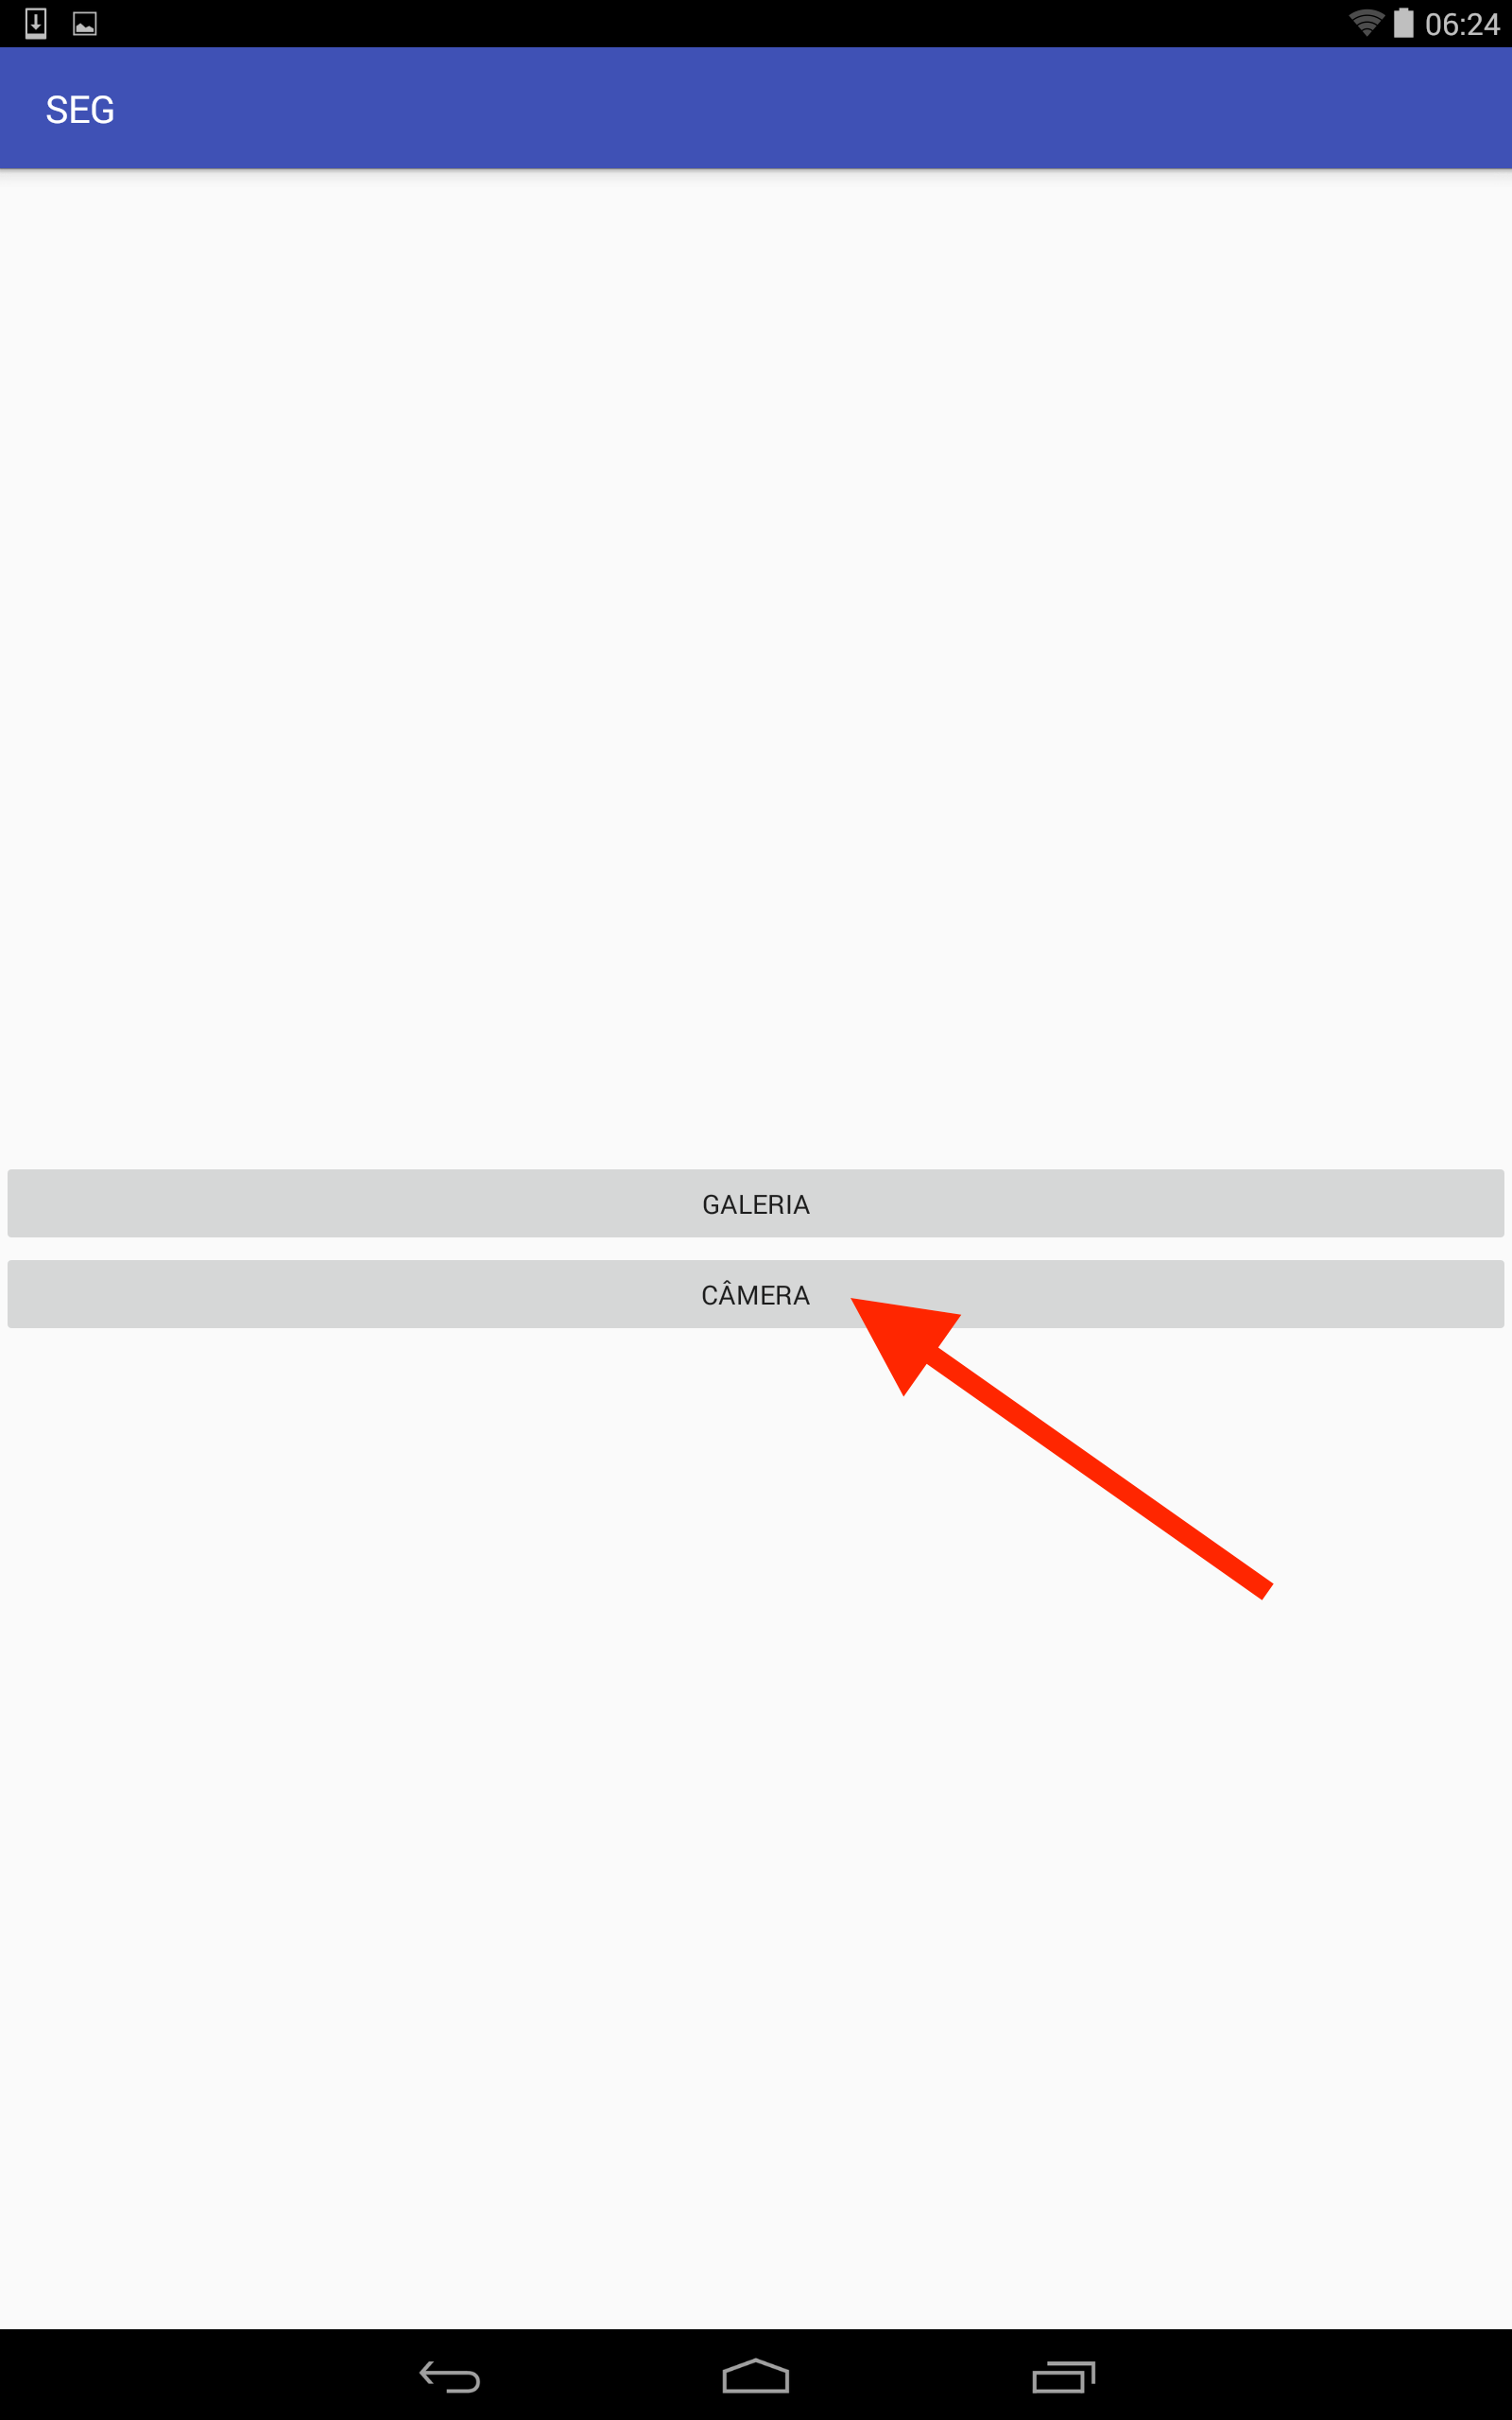
\includegraphics[width=0.4\columnwidth]{img/camera_app_n1.png}
           \caption{\label{fig:camera_app_p1}Sequência de atividades para aquisição e tratamento das imagens por meio da câmera do dispositivo.}
           % \vspace{2.0em}
       \end{center}
   \end{figure}
% Figura 
\begin{figure}[!htb]
 \centering
 \def\baselinestretch{1}\small\normalsize
 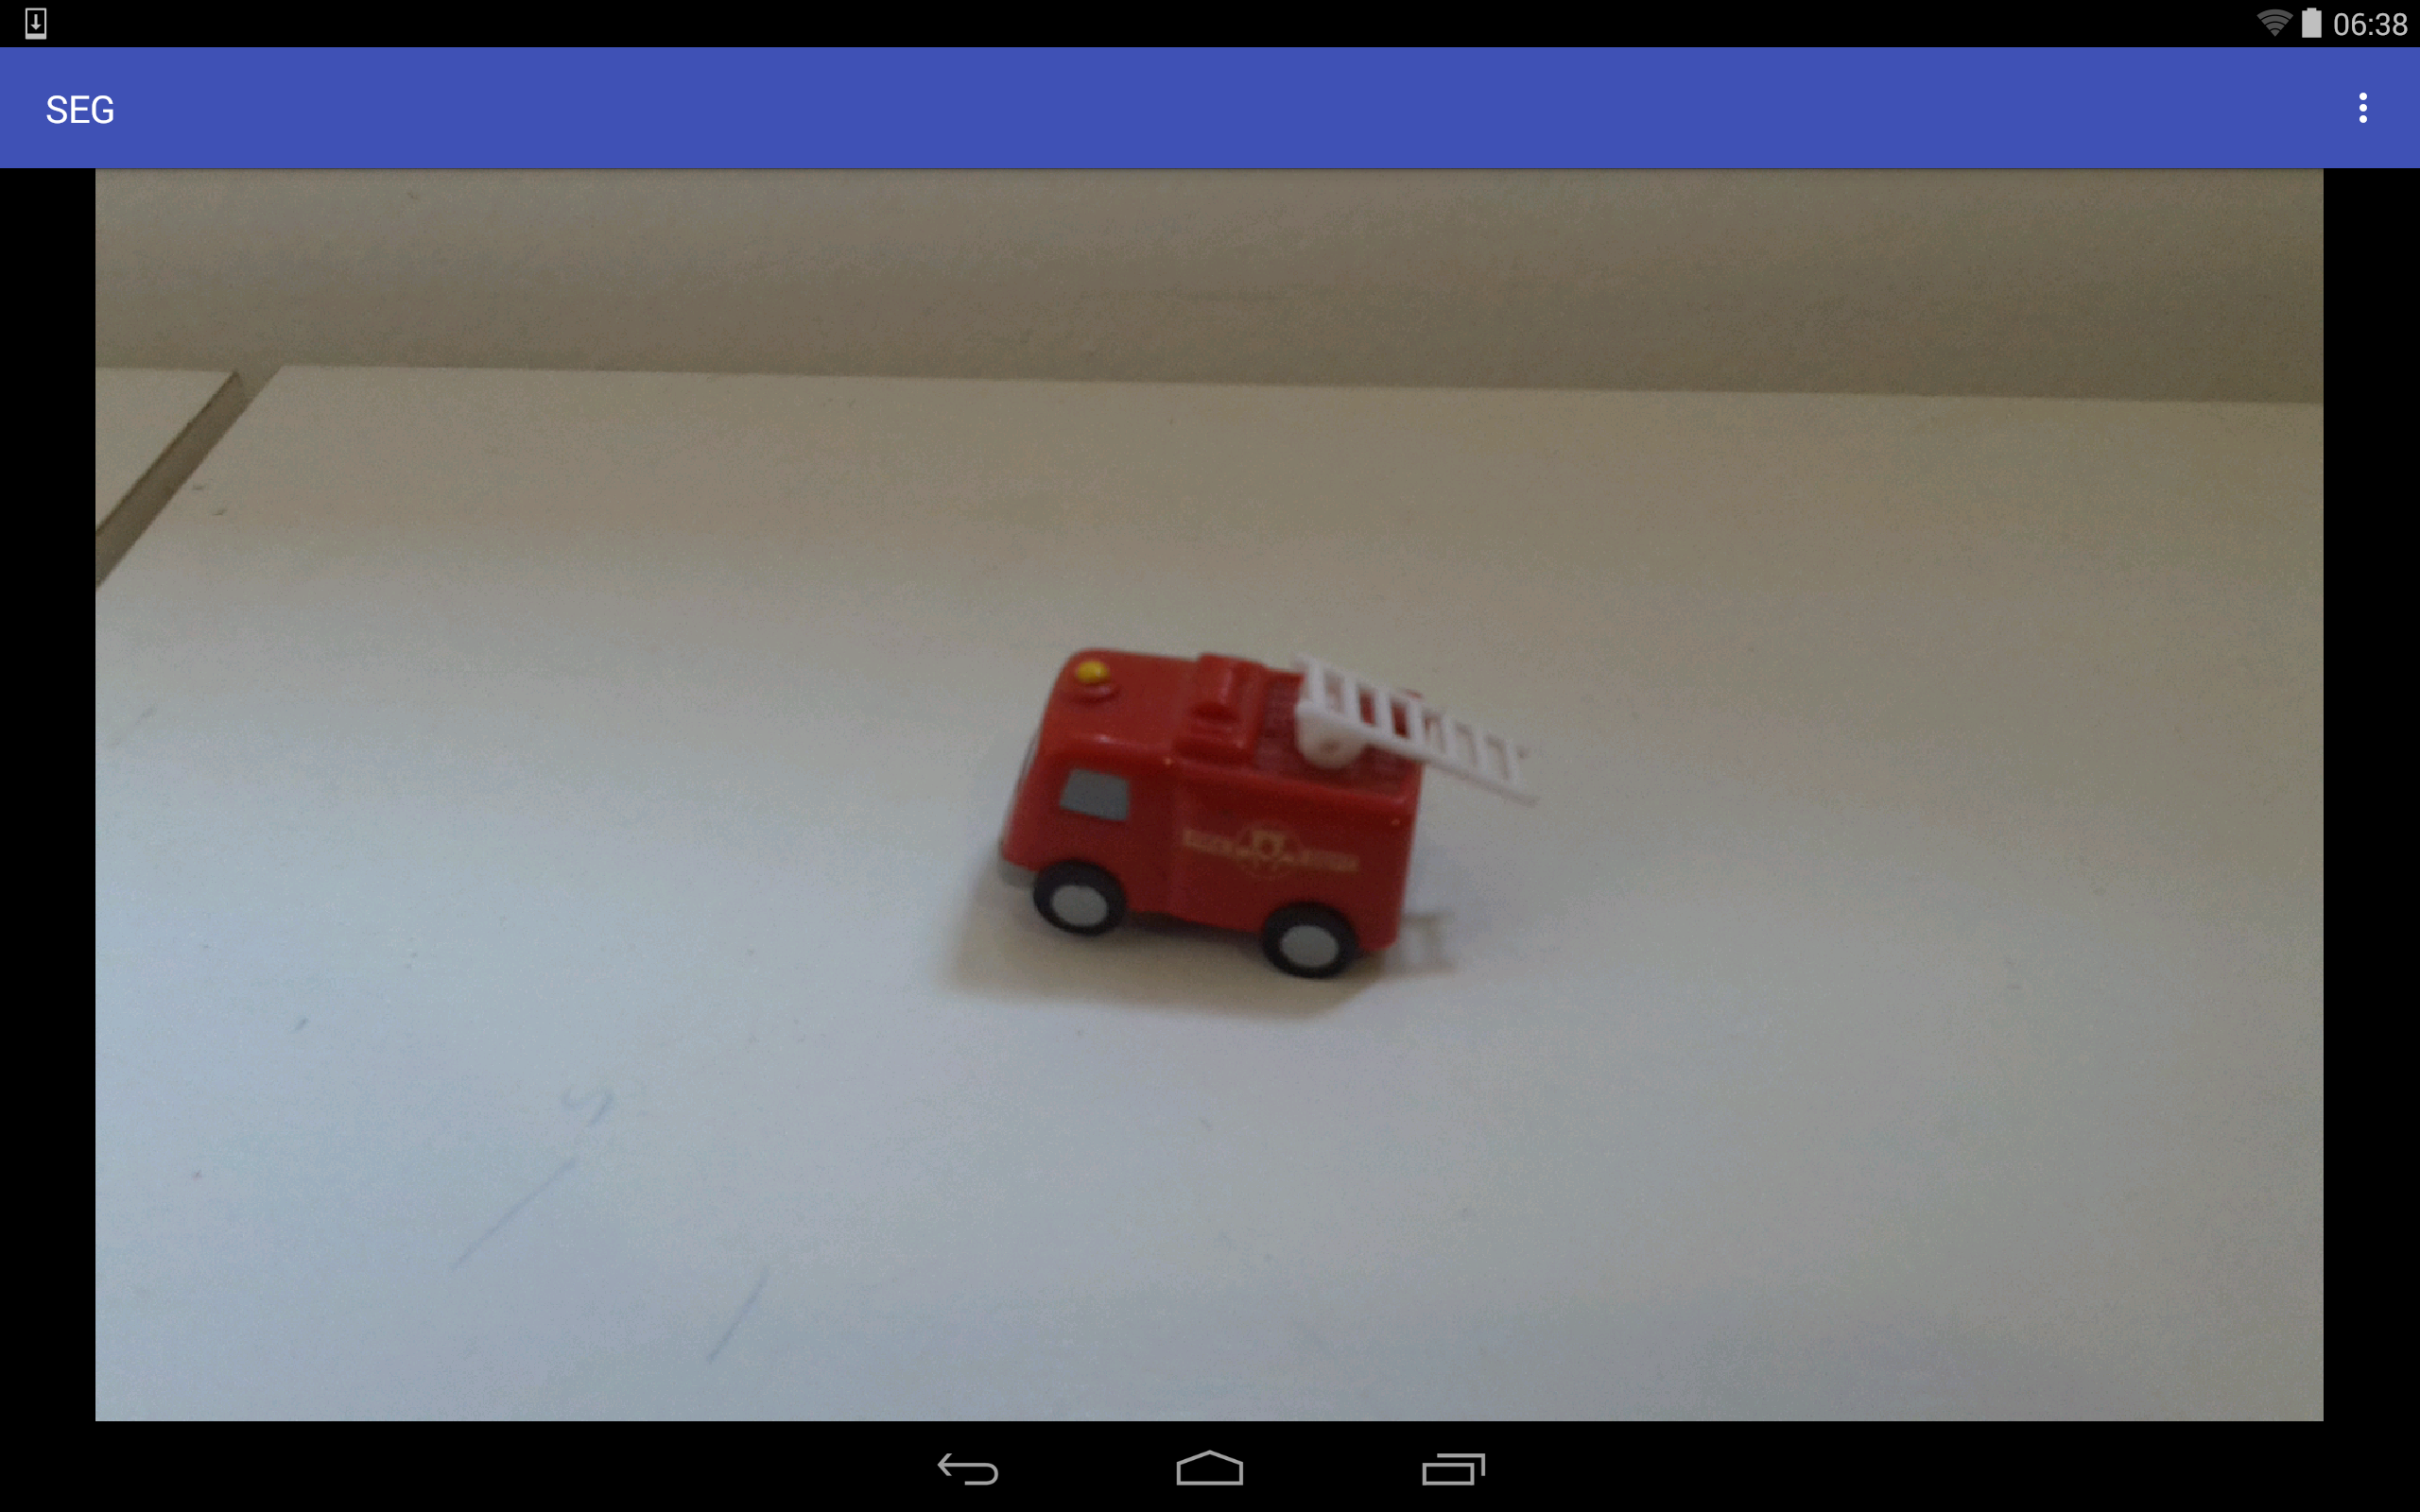
\includegraphics[width=0.4\textwidth]{img/camera_app_n2.png}\qquad
 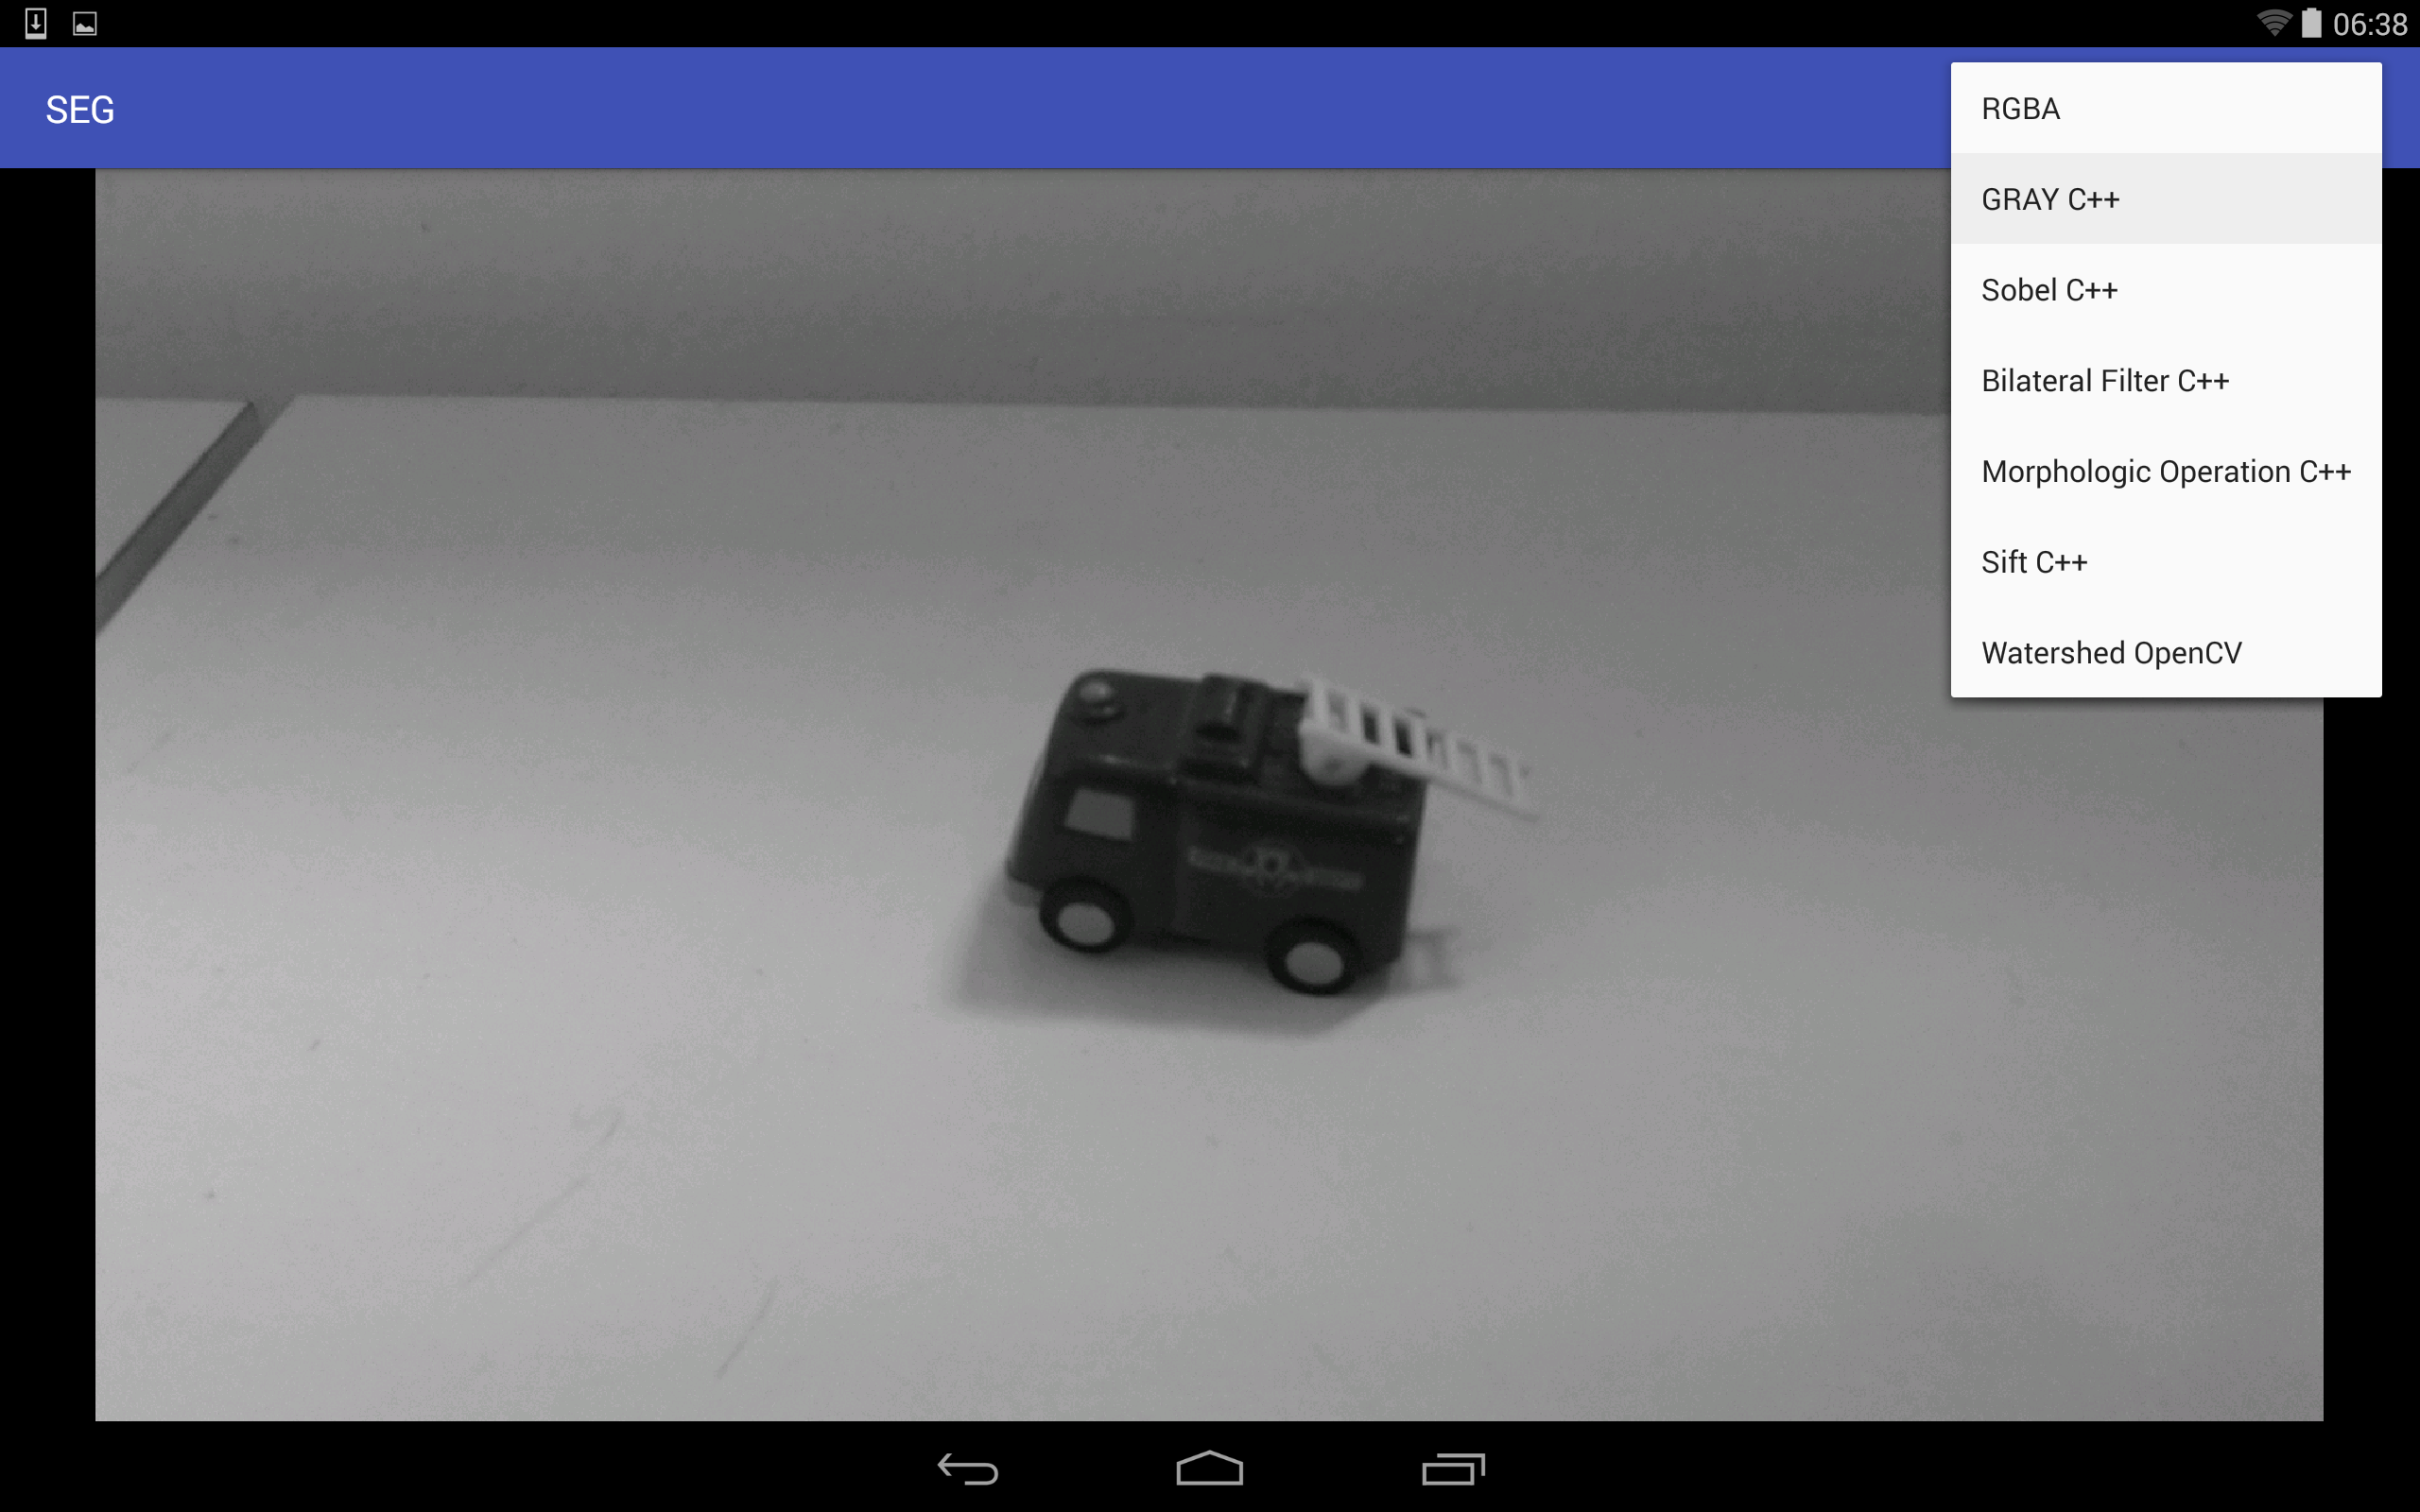
\includegraphics[width=0.4\textwidth]{img/camera_app_n3.png} 
 \caption{\label{fig:camera_app_p2}Sequência de atividades para aquisição e tratamento das imagens por meio da câmera do dispositivo.}
 %\vspace{2.0em}
\end{figure}
% Figura 
\begin{figure}[!htb]
 \centering
 \def\baselinestretch{1}\small\normalsize
 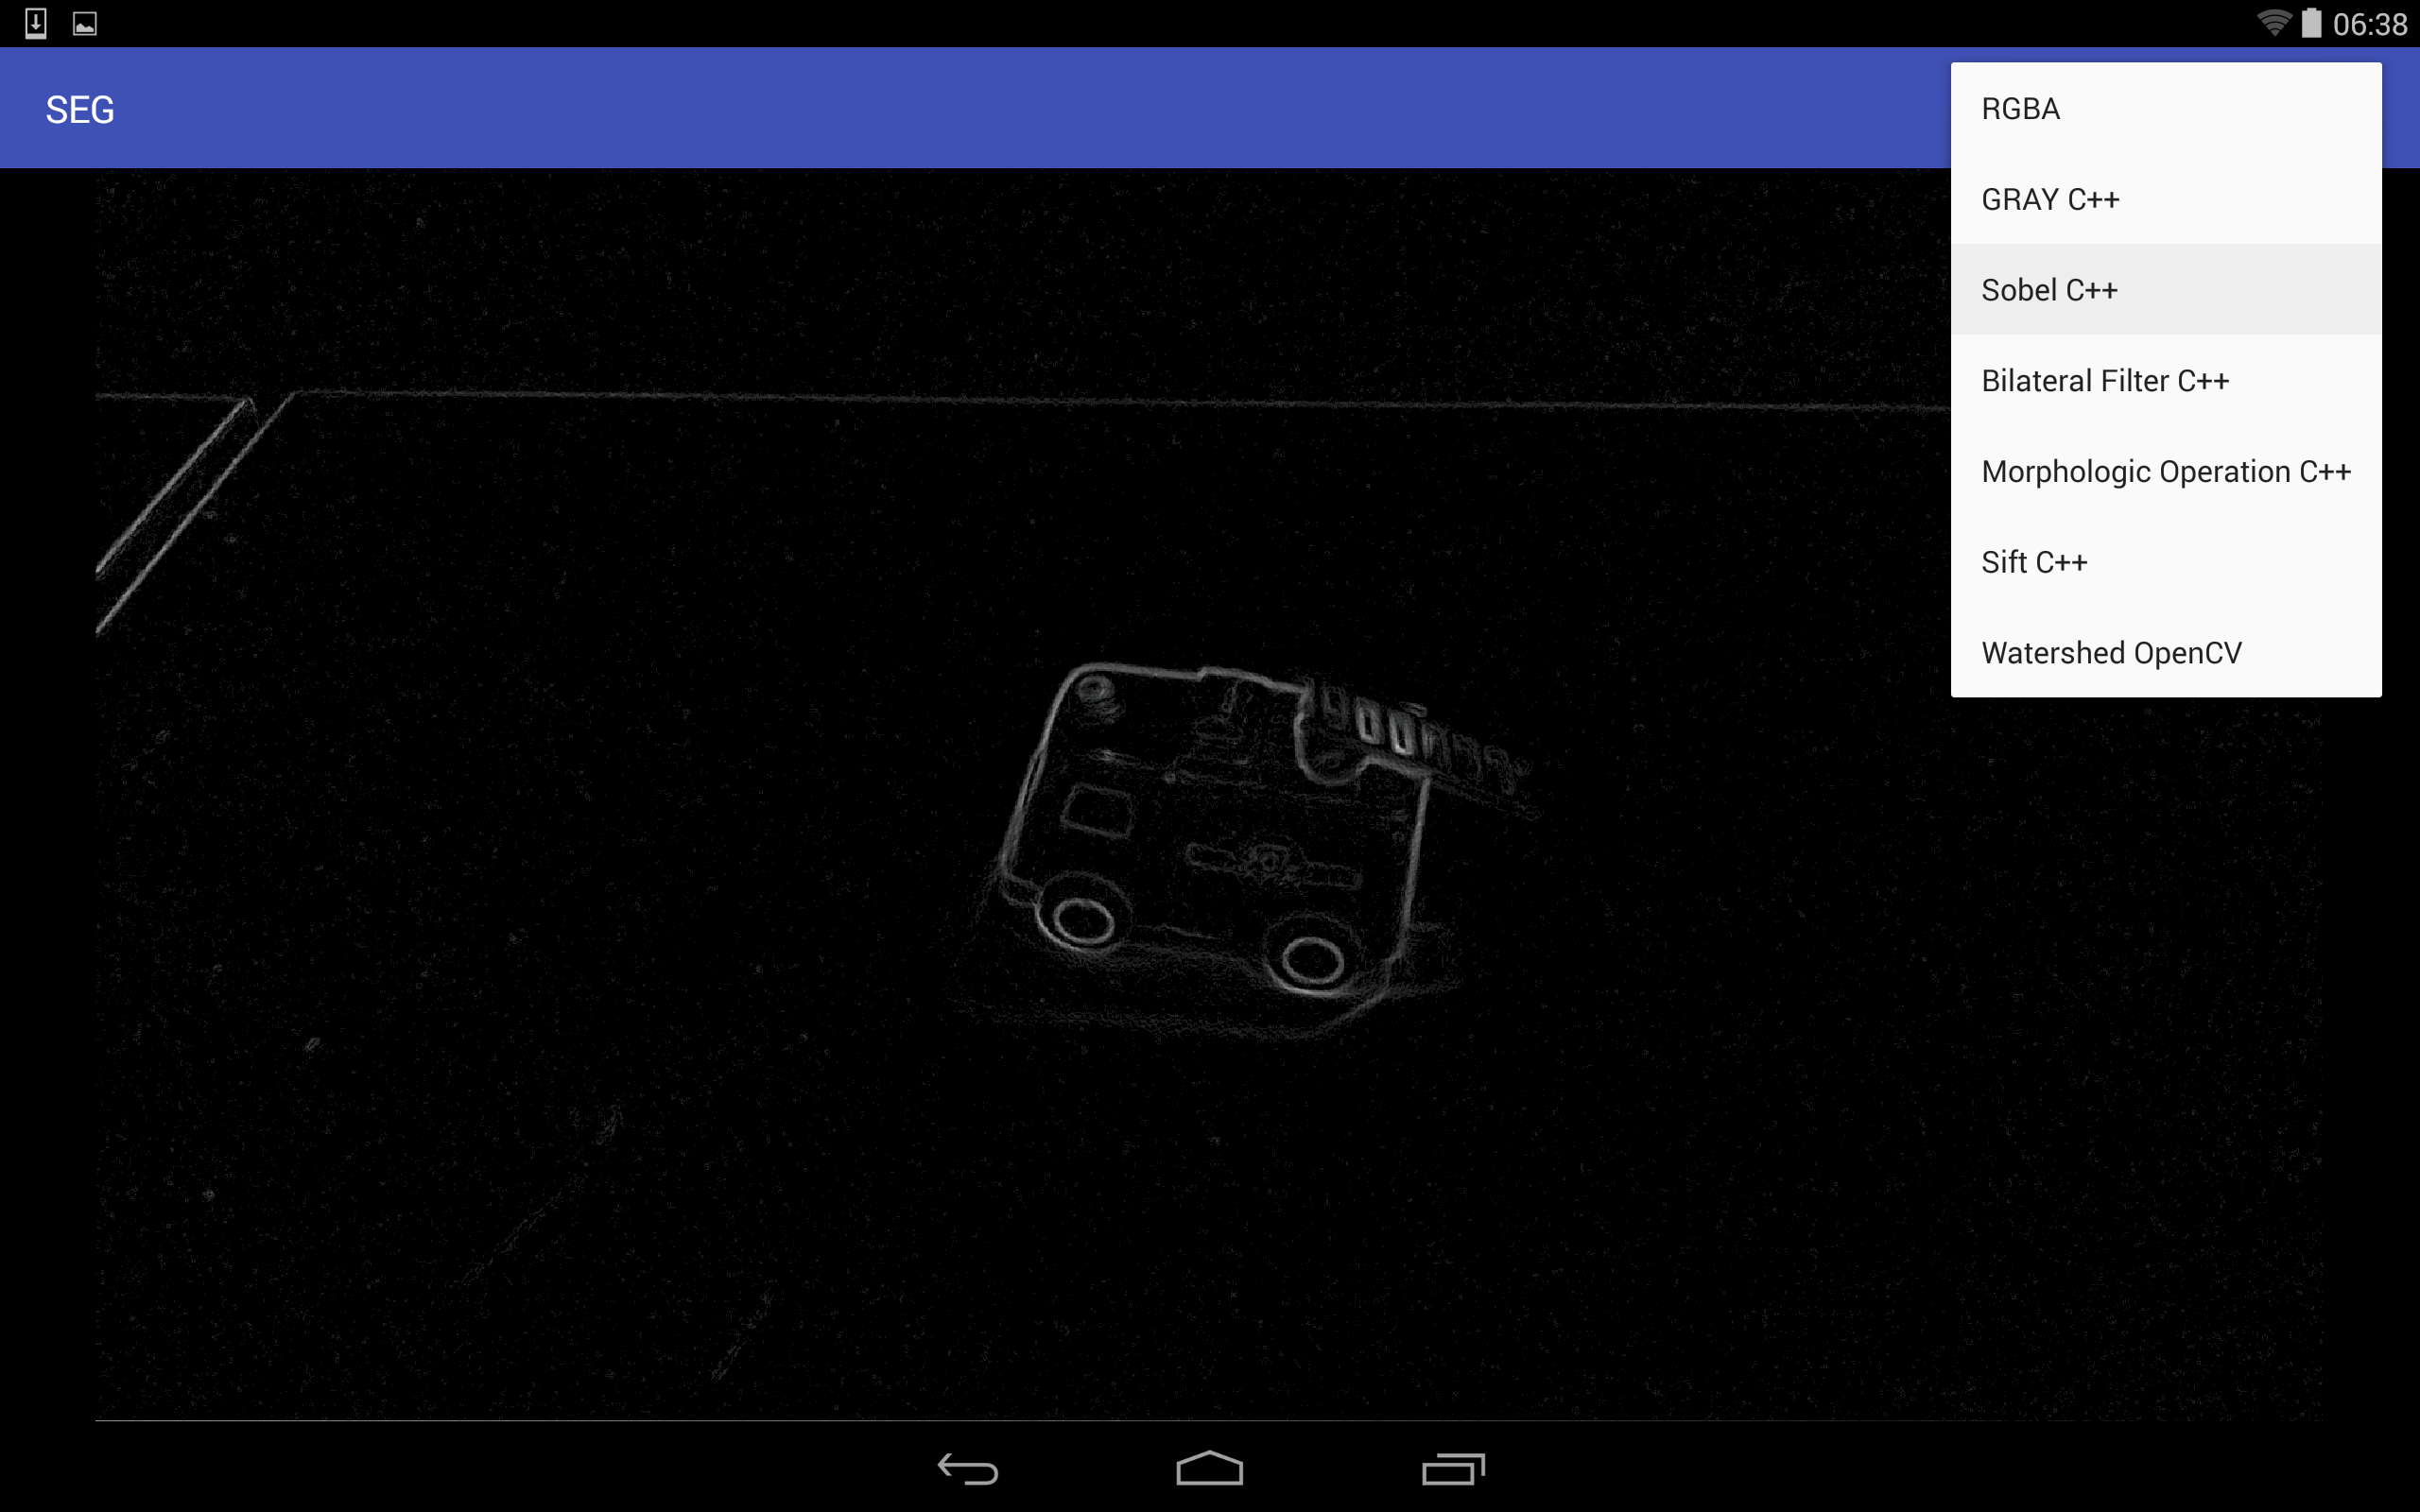
\includegraphics[width=0.4\textwidth]{img/camera_app_n4.png}\qquad
 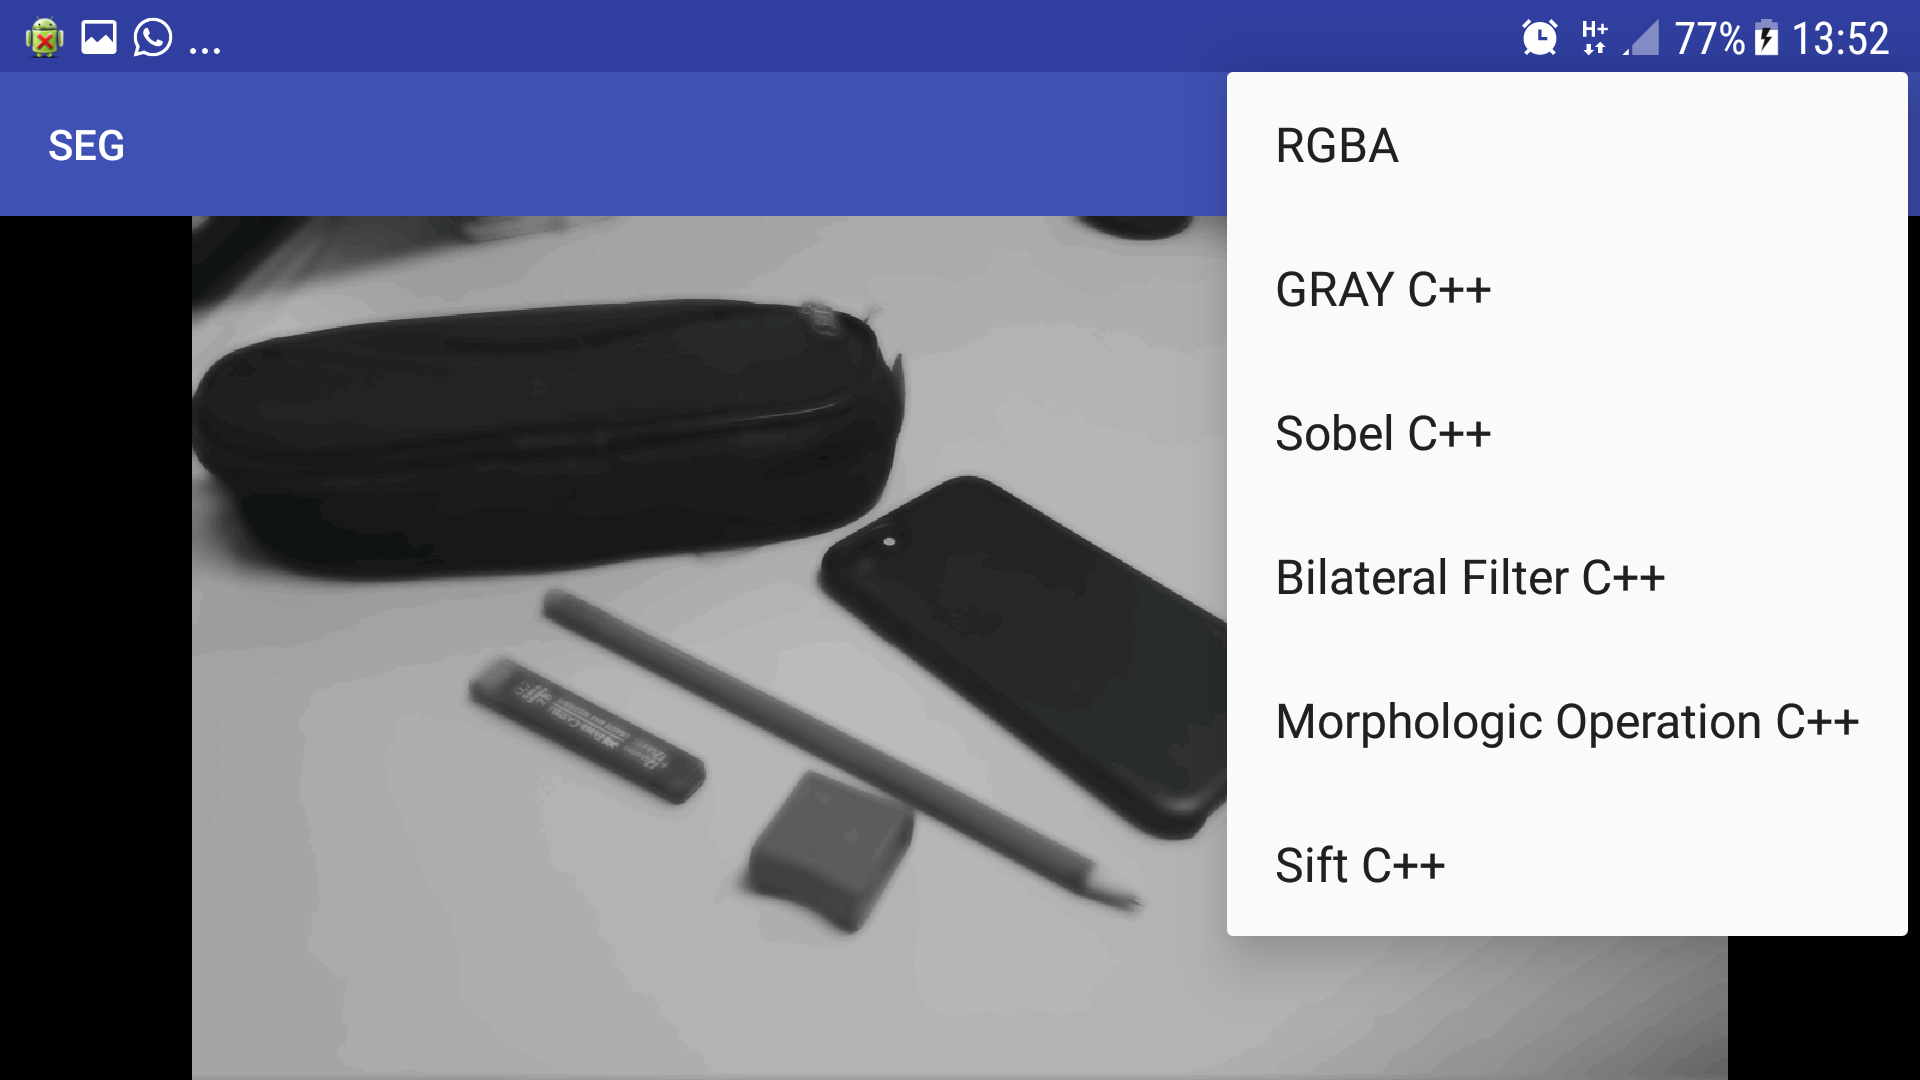
\includegraphics[width=0.4\textwidth]{img/camera_app_n5.png} 
 \caption{\label{fig:camera_app_p3}Sequência de atividades para aquisição e tratamento das imagens por meio da câmera do dispositivo.}
 %\vspace{2.0em}
\end{figure}
% Figura 
\begin{figure}[!htb]
 \centering
 \def\baselinestretch{1}\small\normalsize
 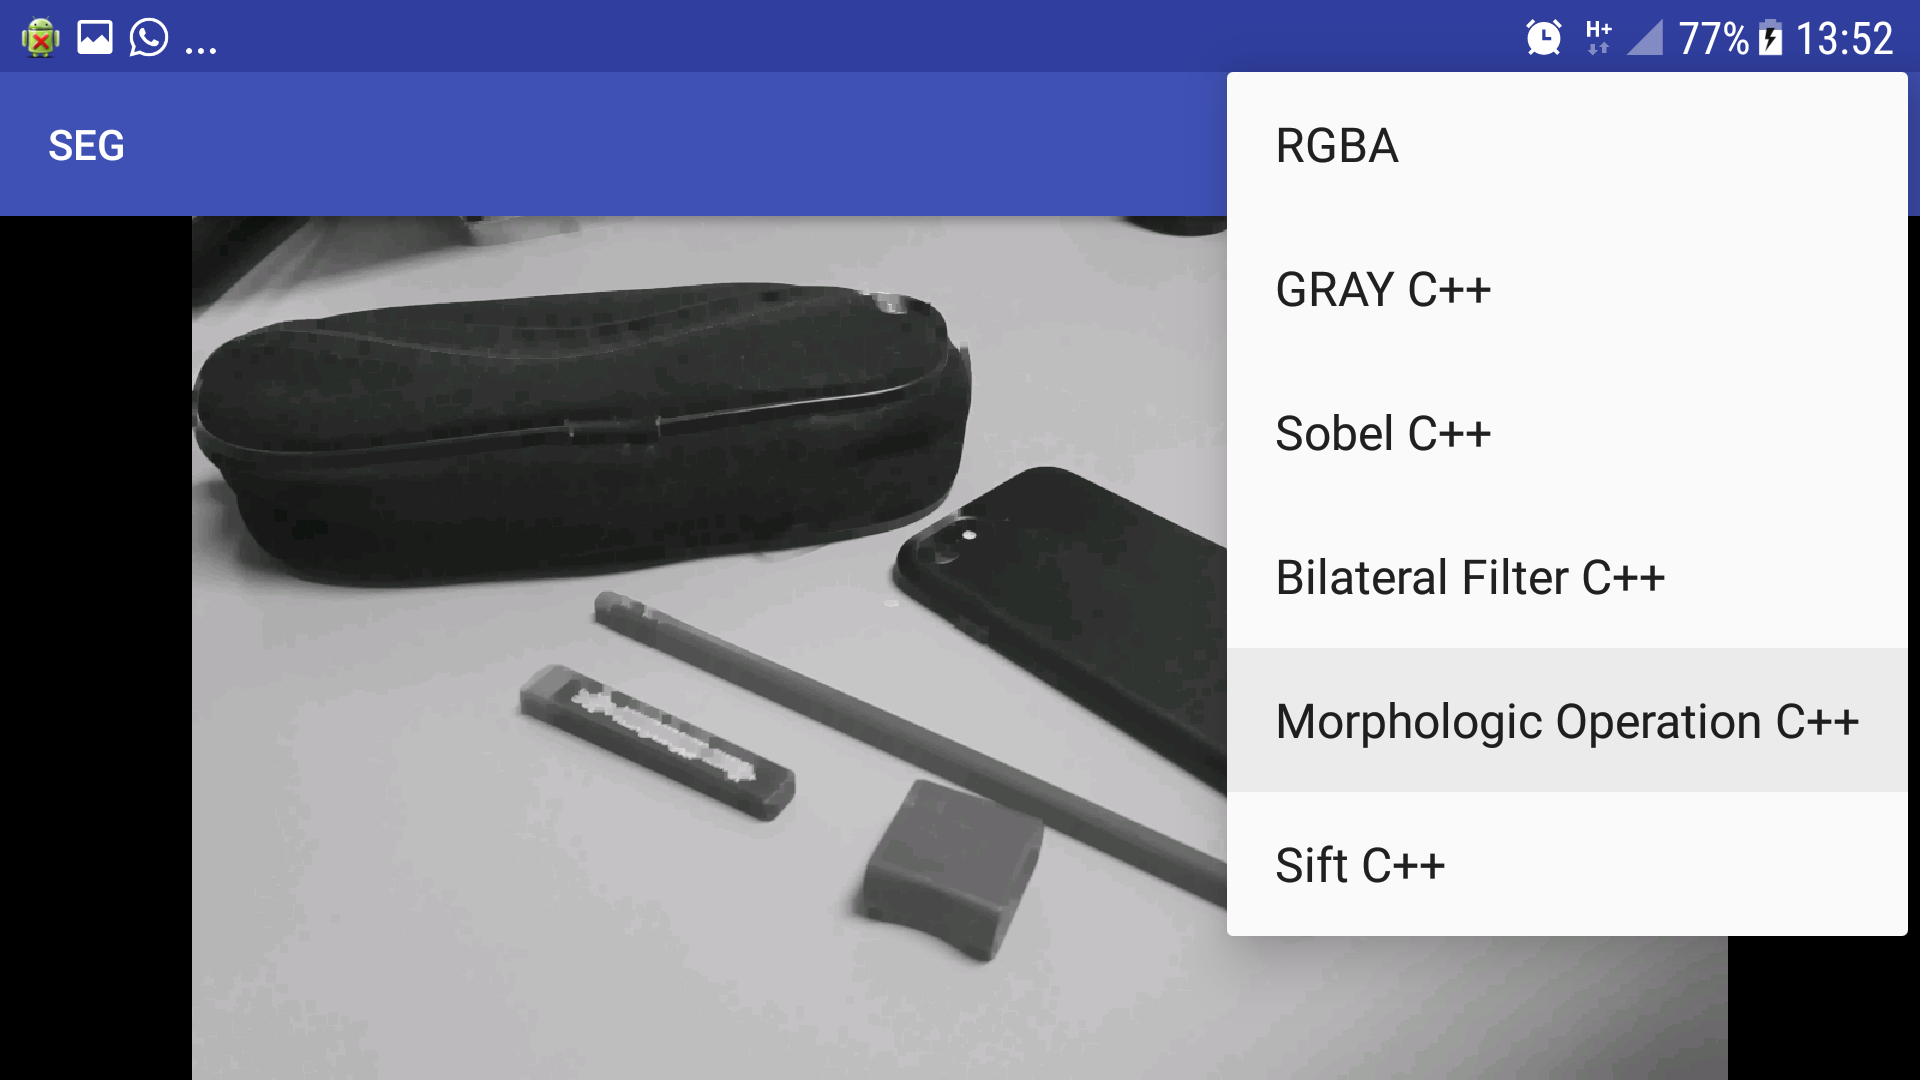
\includegraphics[width=0.4\textwidth]{img/camera_app_n6.png}\qquad
 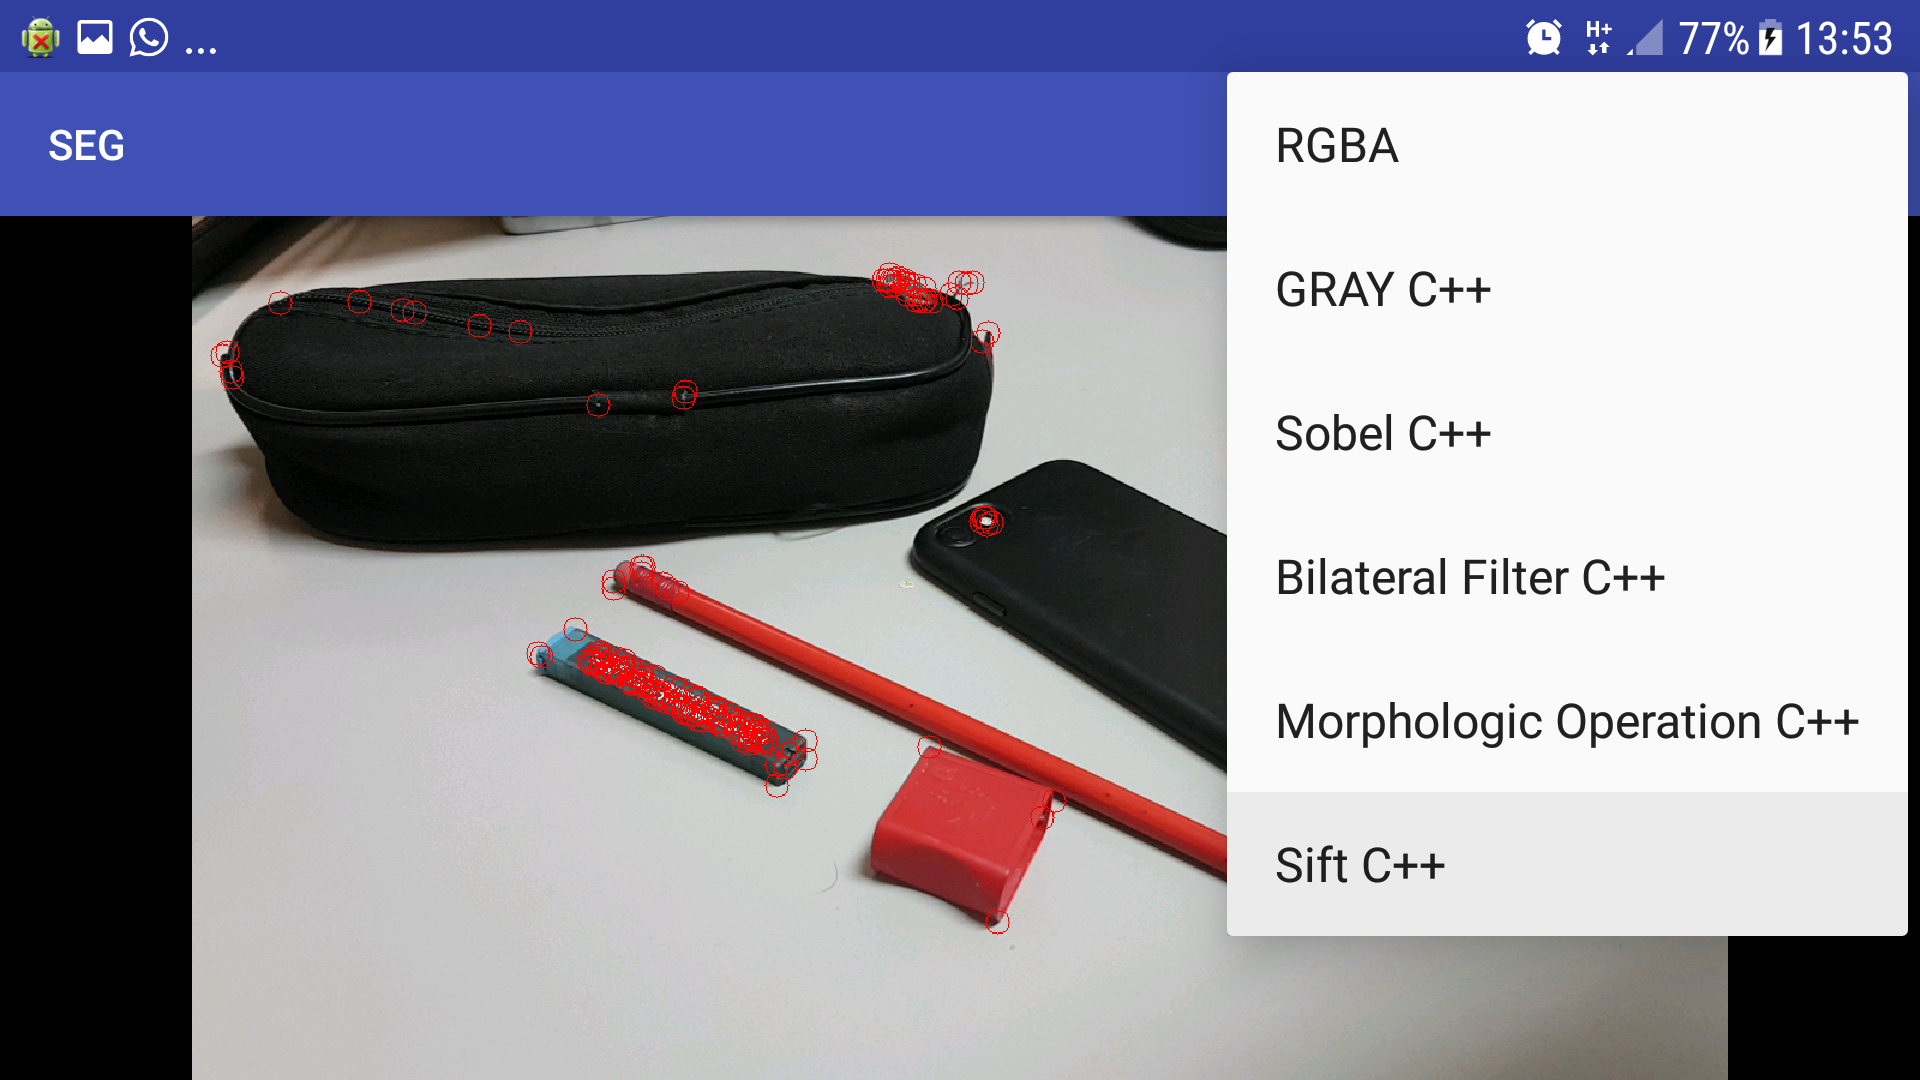
\includegraphics[width=0.4\textwidth]{img/camera_app_n7.png} 
 \caption{\label{fig:camera_app_p4}Sequência de atividades para aquisição e tratamento das imagens por meio da câmera do dispositivo.}
 %\vspace{2.0em}
\end{figure}
\clearpage

\section{Segmentação da imagem}\label{sec:segmentacao_aplicacao}

A segmentação da imagem, é feita por meio do algoritmo desenvolvido para esta aplicação.

\subsection{\textit{Watershed} Desenvolvido}

Após a escolha da imagem, ao clicar sobre o botão "\textit{watershed}", a imagem escolhida será segmentada de acordo com o algoritmo desenvolvido neste projeto. Antes disso, pode-se ainda ajustar os parâmetros do Filtro Bilateral e do Operador Sobel por meio de dois \textit{seekbars}. A sequência de \textit{steps} apresentados na seção \ref{sec:alg} do capítulo \ref{cap:algoritmo} é executada pelo processador do dispositivo utilizado e o resultado da imagem segmentada é apresentada na tela.

A seguir são exibidos os resultados da segmentação para algumas das imagens testadas.
% Figura 
\begin{figure}[!htb]
 \centering
 \def\baselinestretch{1}\small\normalsize
 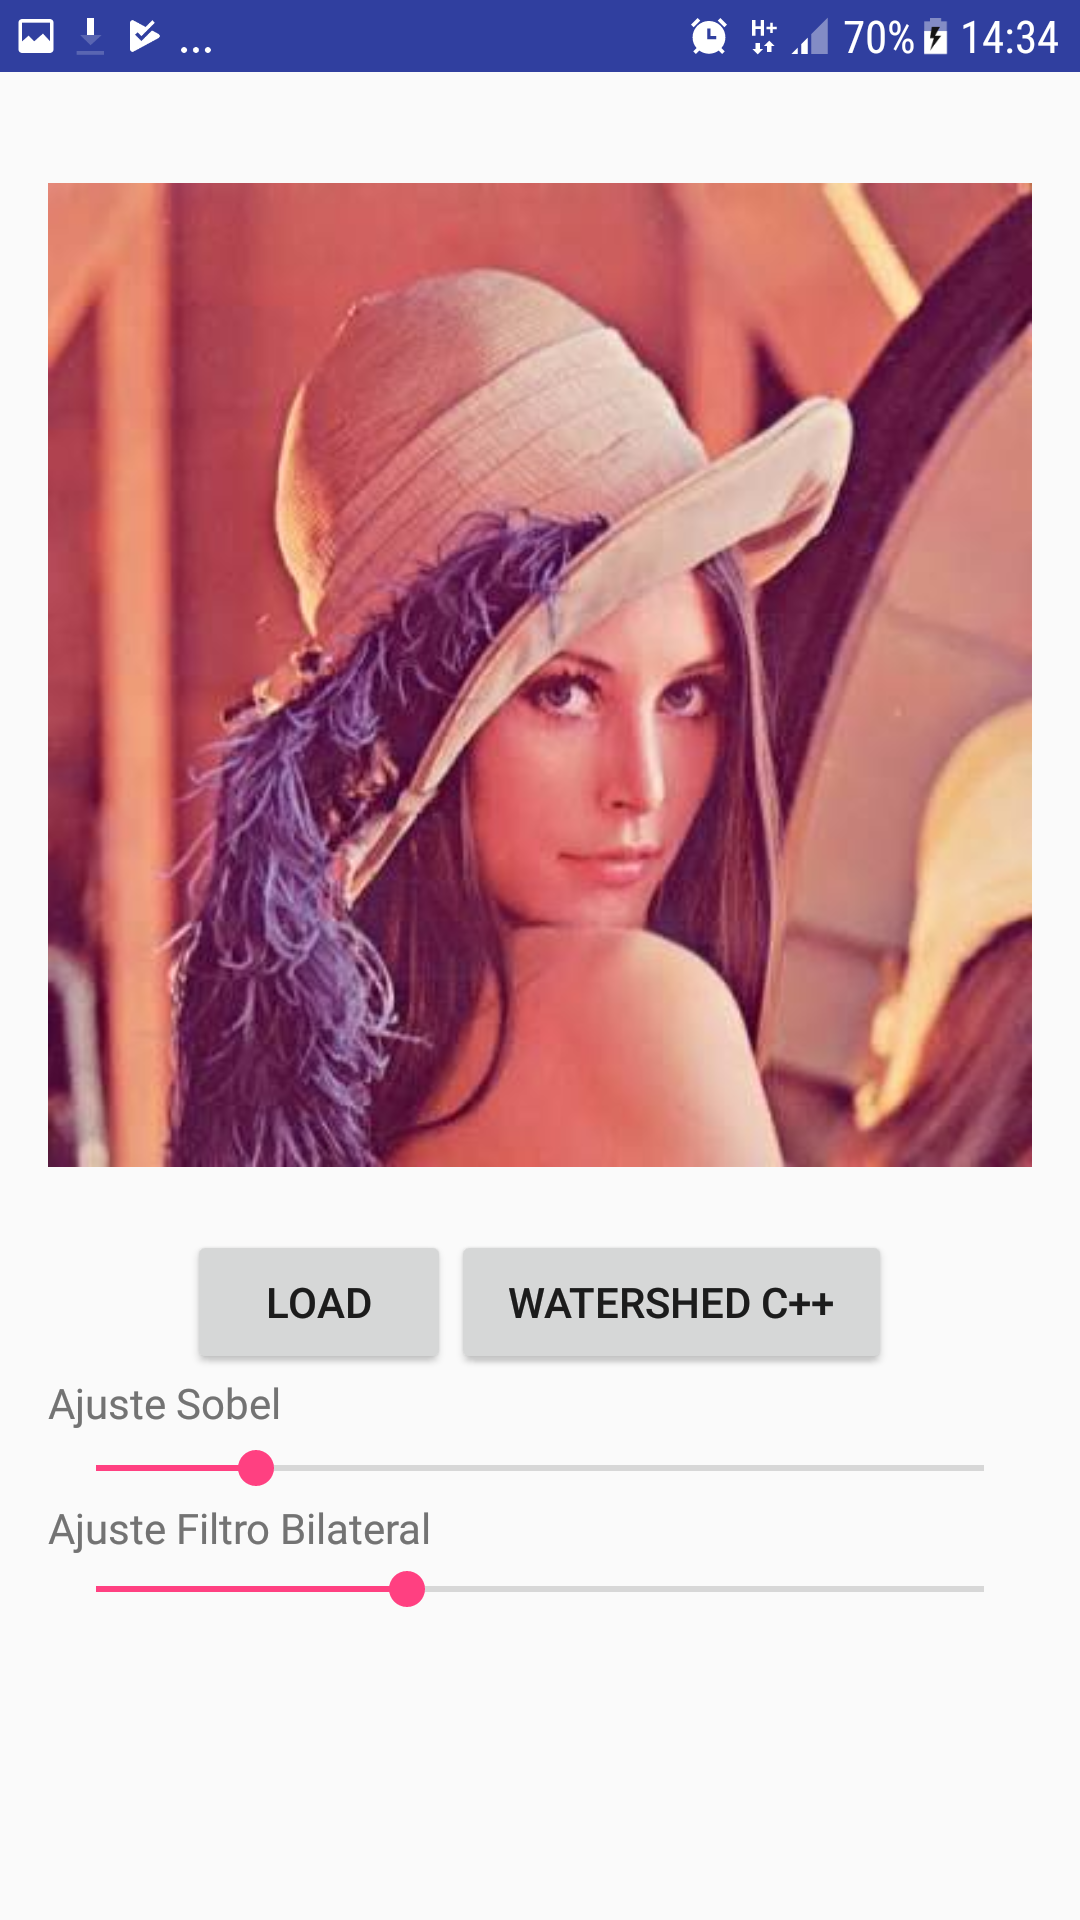
\includegraphics[width=0.4\textwidth]{img/imagem_watershed_desenvolvido_app_n1.png}\qquad
 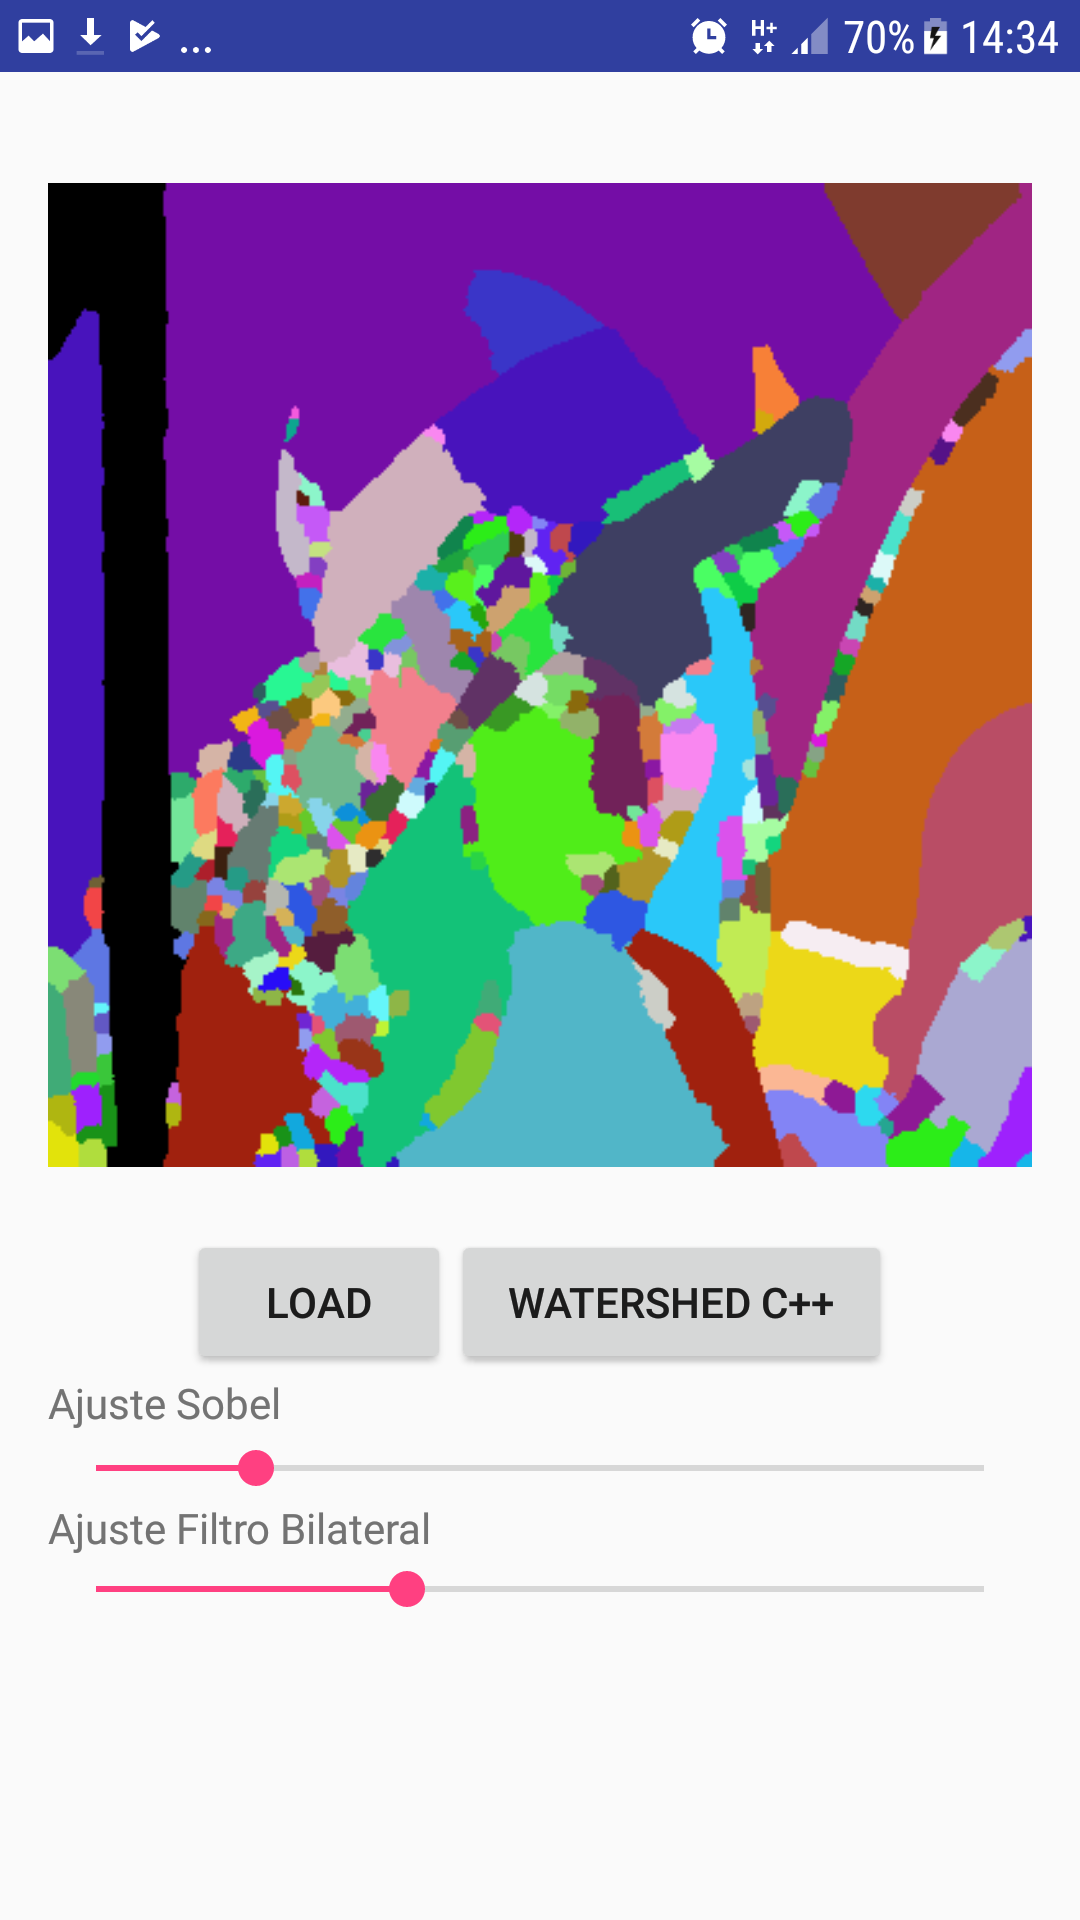
\includegraphics[width=0.4\textwidth]{img/resultado_watershed_desenvolvido_app_n1.png} 
 \caption{\label{fig:resultado_watershed_desenvolvido_app_p1}Resultados de segmentação utilizando o algoritmo \textit{watershed} desenvolvido.}
 %\vspace{2.0em}
\end{figure}
% Figura 
\begin{figure}[!htb]
 \centering
 \def\baselinestretch{1}\small\normalsize
 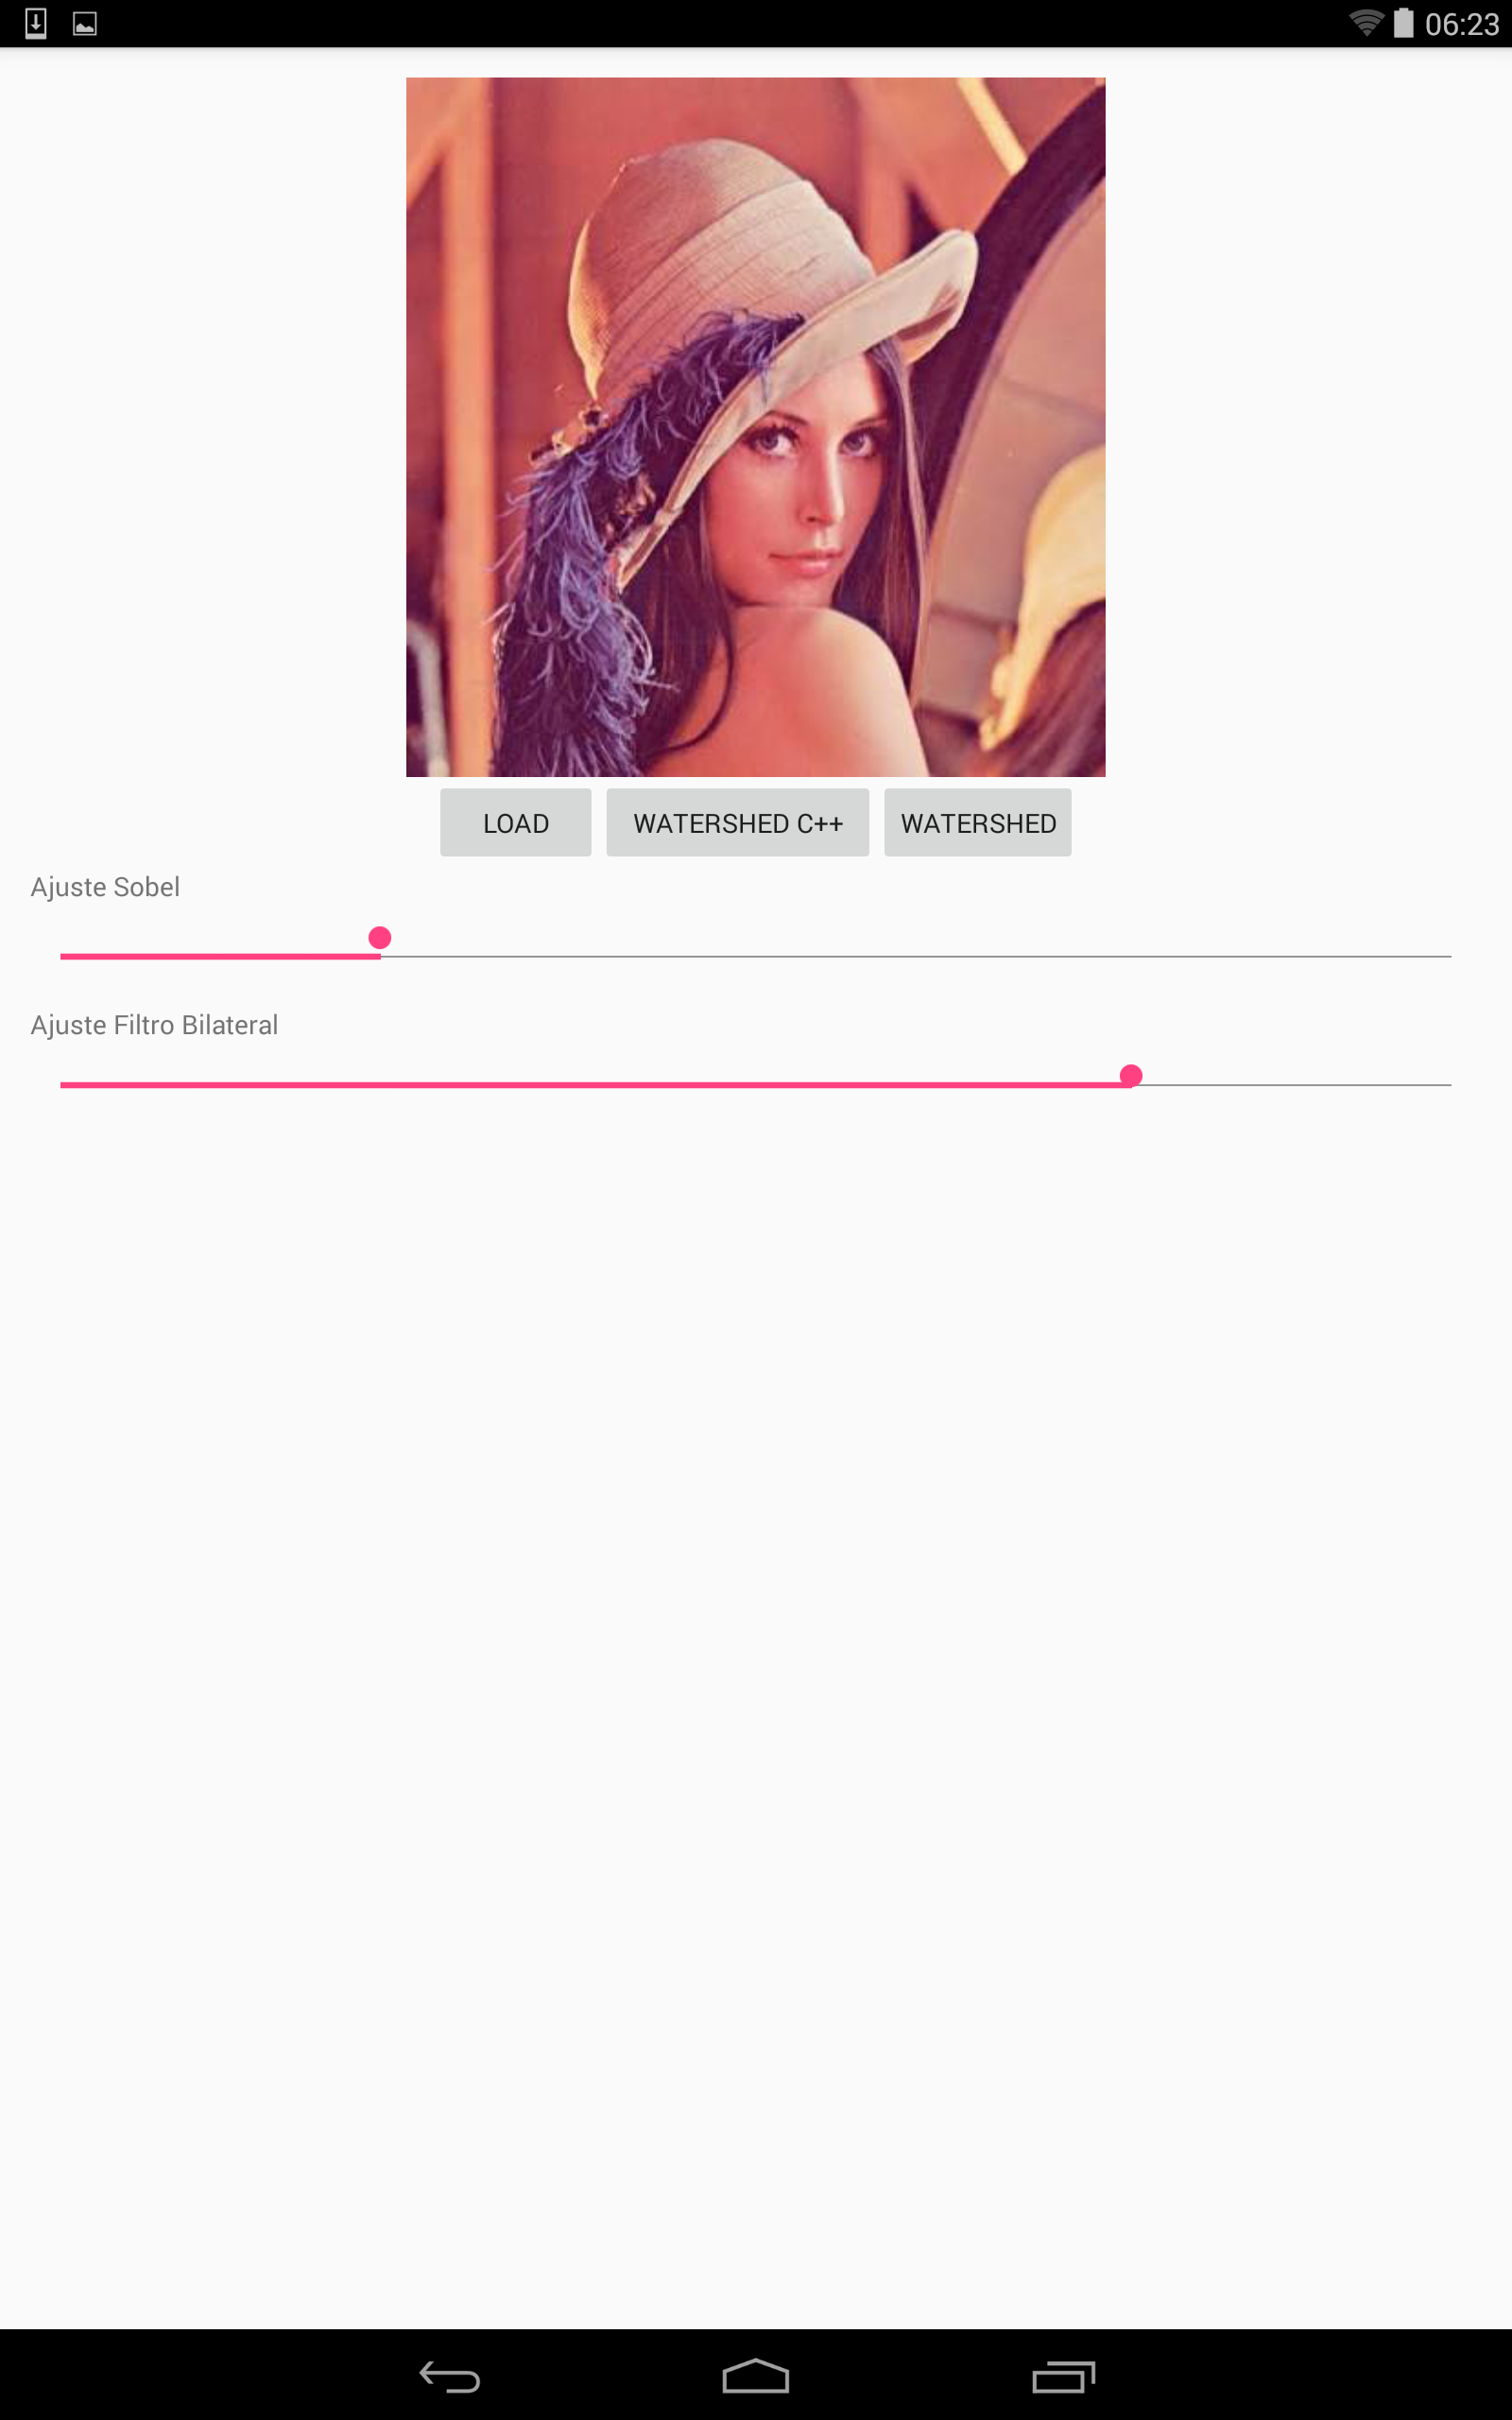
\includegraphics[width=0.4\textwidth]{img/galeria_app_n4.png}\qquad
 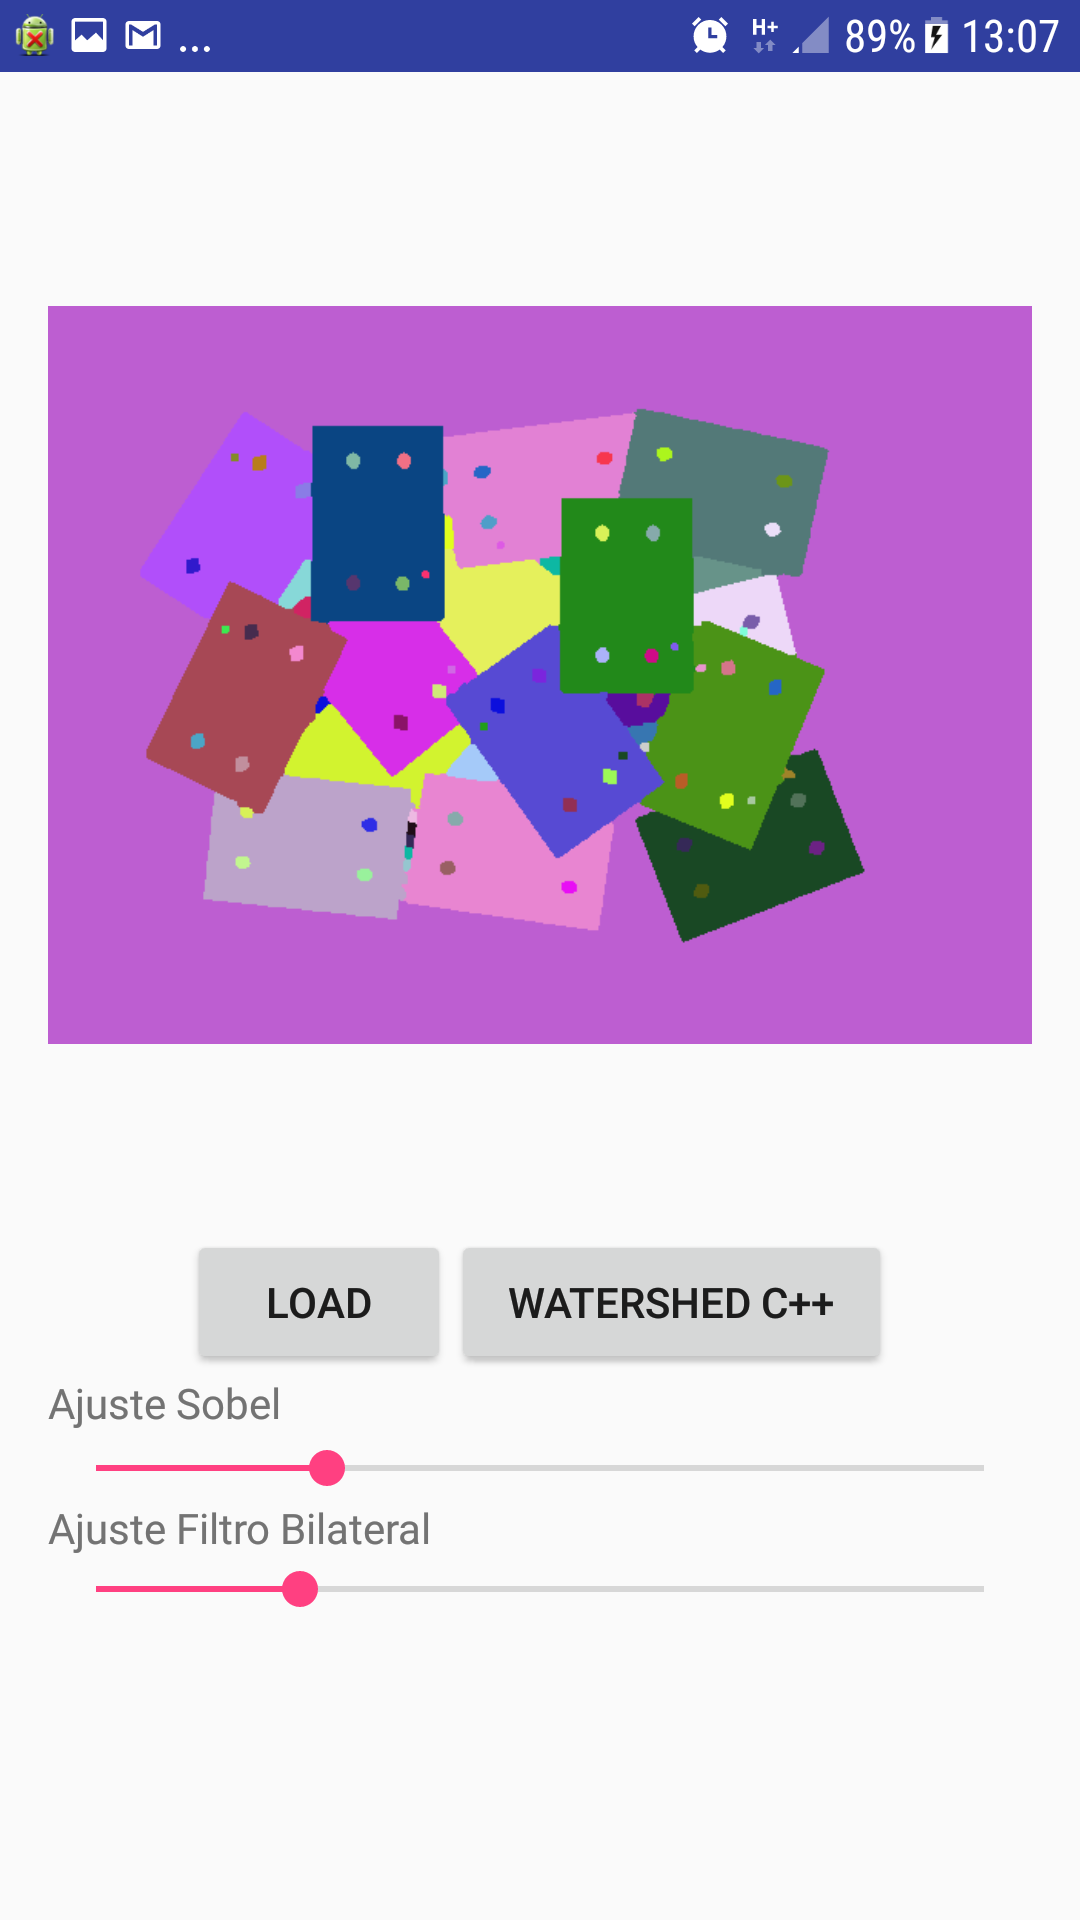
\includegraphics[width=0.4\textwidth]{img/resultado_watershed_desenvolvido_app_n2.png} 
 \caption{\label{fig:resultado_watershed_desenvolvido_app_p2}Resultados de segmentação utilizando o algoritmo \textit{watershed} desenvolvido.}
 %\vspace{2.0em}
\end{figure}
% Figura 
\begin{figure}[!htb]
 \centering
 \def\baselinestretch{1}\small\normalsize
 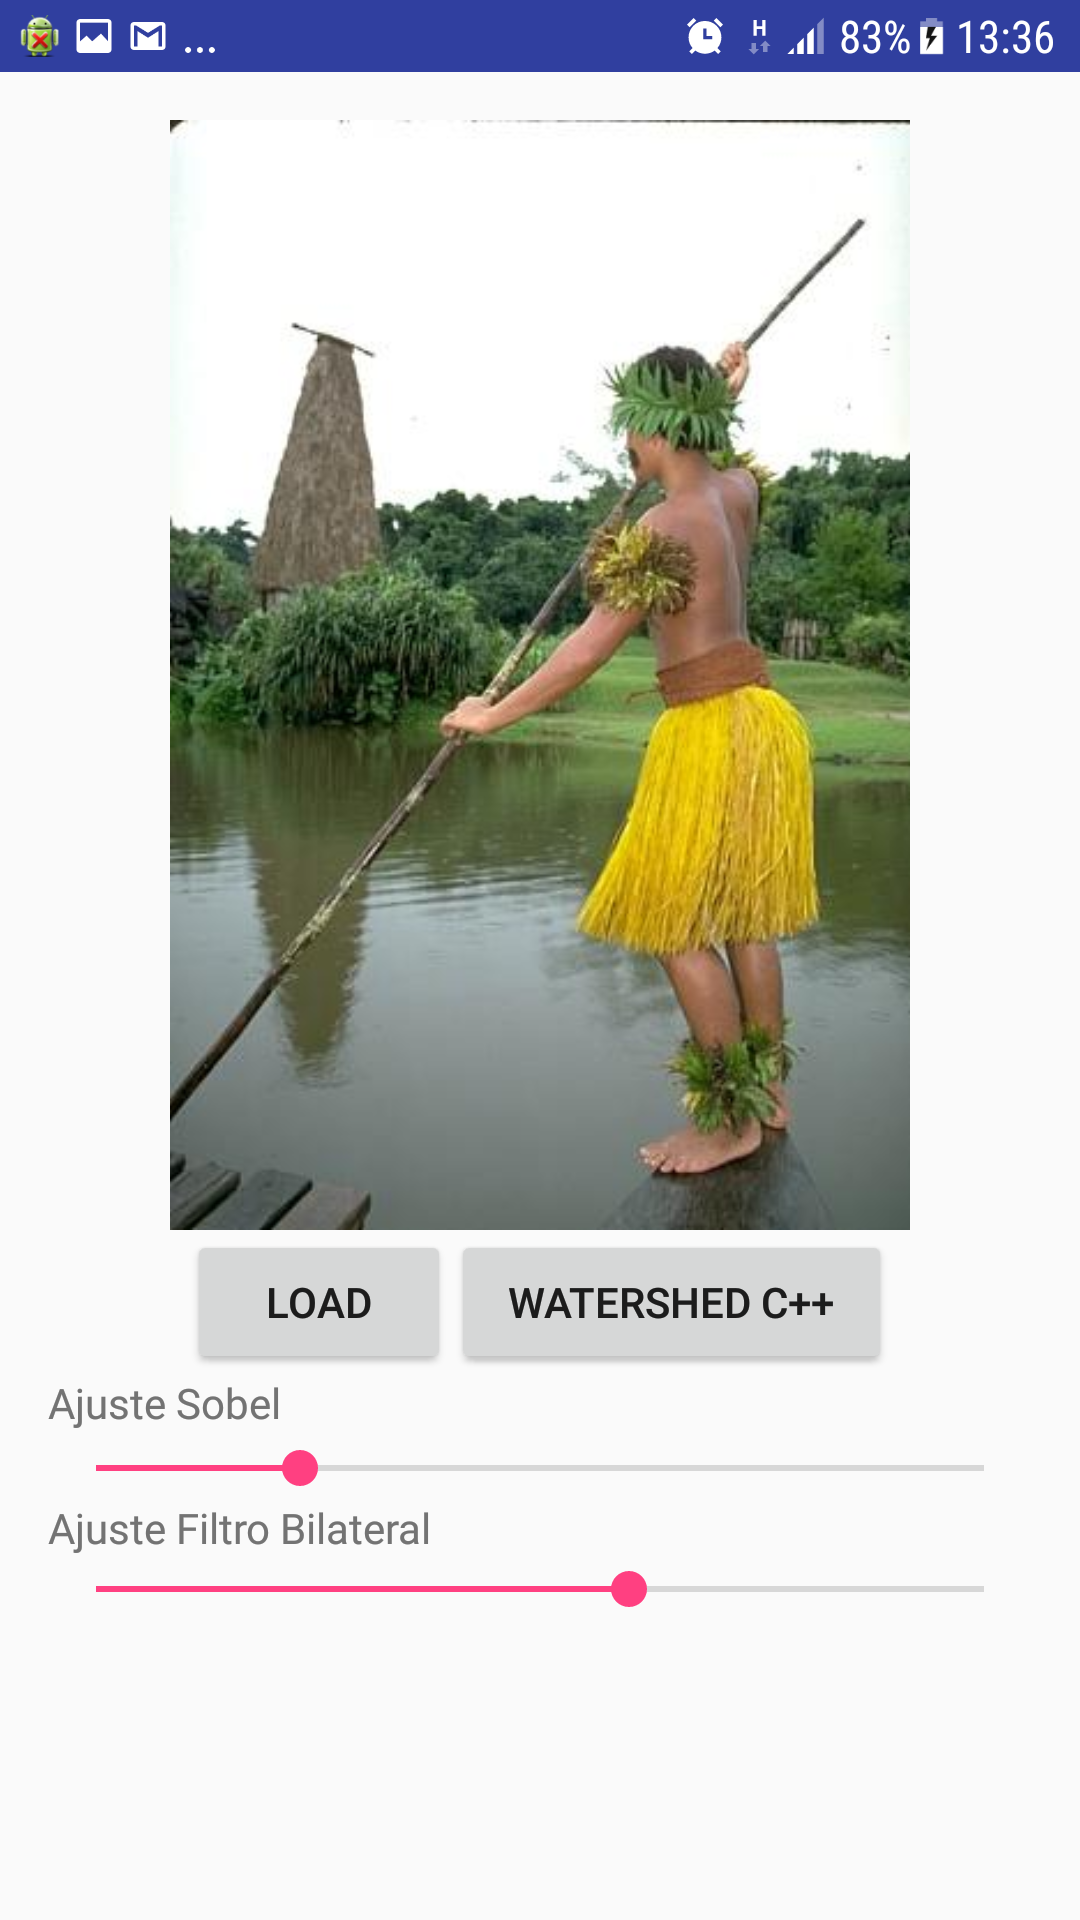
\includegraphics[width=0.4\textwidth]{img/imagem_watershed_desenvolvido_app_n3.png}\qquad
 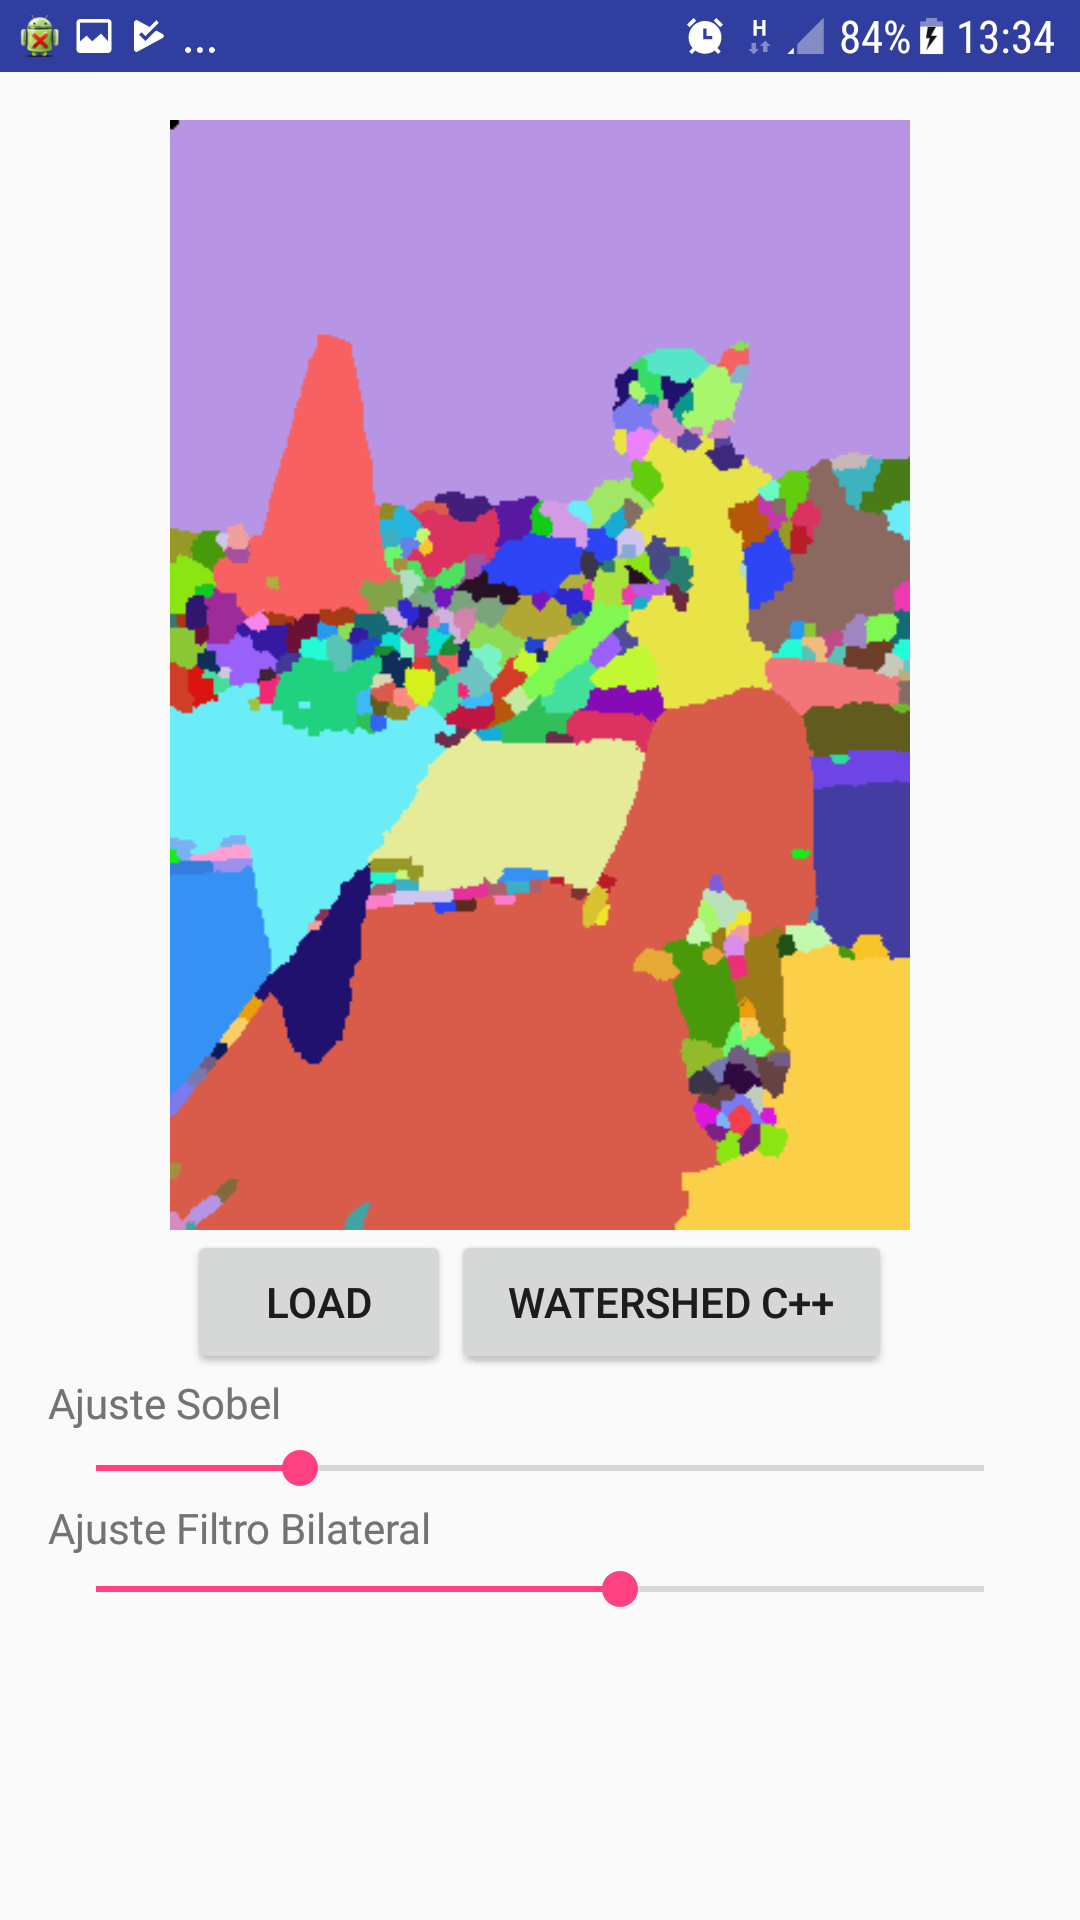
\includegraphics[width=0.4\textwidth]{img/resultado_watershed_desenvolvido_app_n3.png} 
 \caption{\label{fig:resultado_watershed_desenvolvido_app_p3}Resultados de segmentação utilizando o algoritmo \textit{watershed} desenvolvido.}
 %\vspace{2.0em}
\end{figure}
% Figura 
\begin{figure}[!htb]
 \centering
 \def\baselinestretch{1}\small\normalsize
 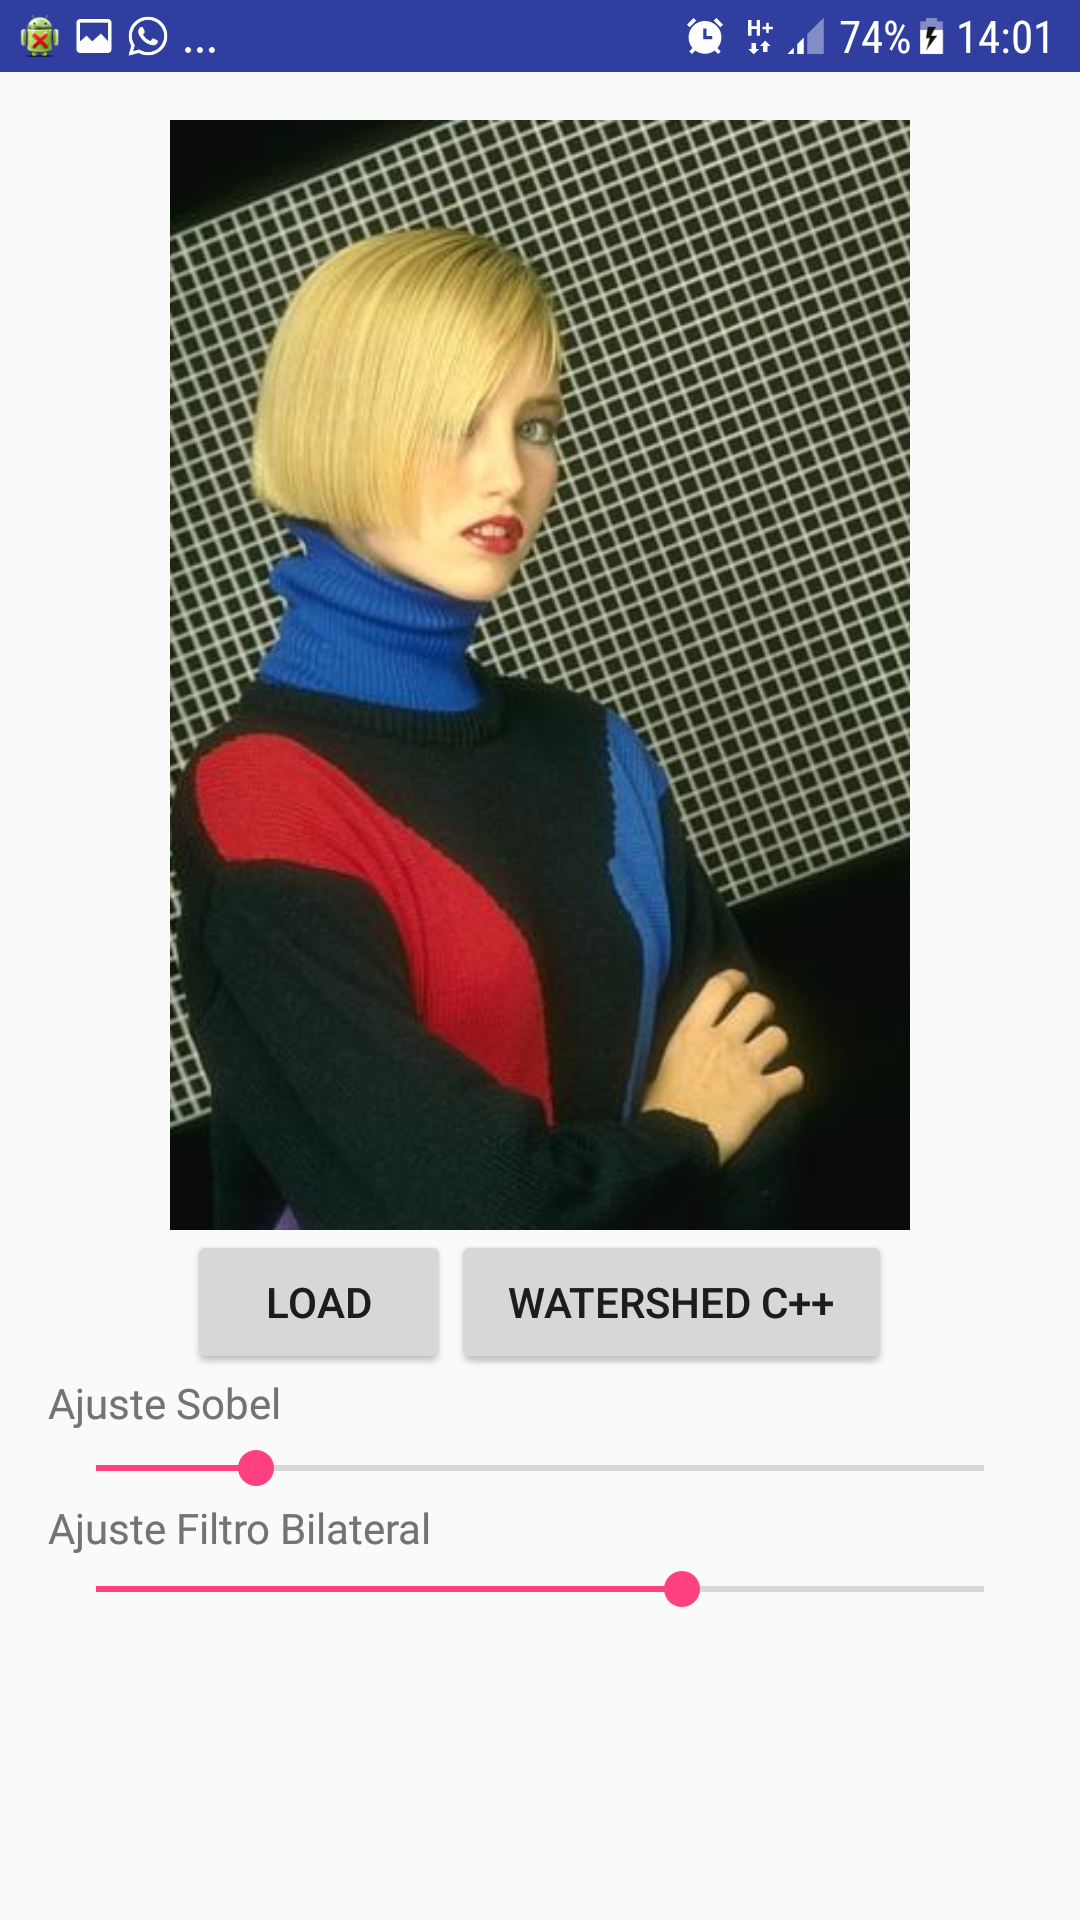
\includegraphics[width=0.4\textwidth]{img/imagem_watershed_desenvolvido_app_n4.png}\qquad
 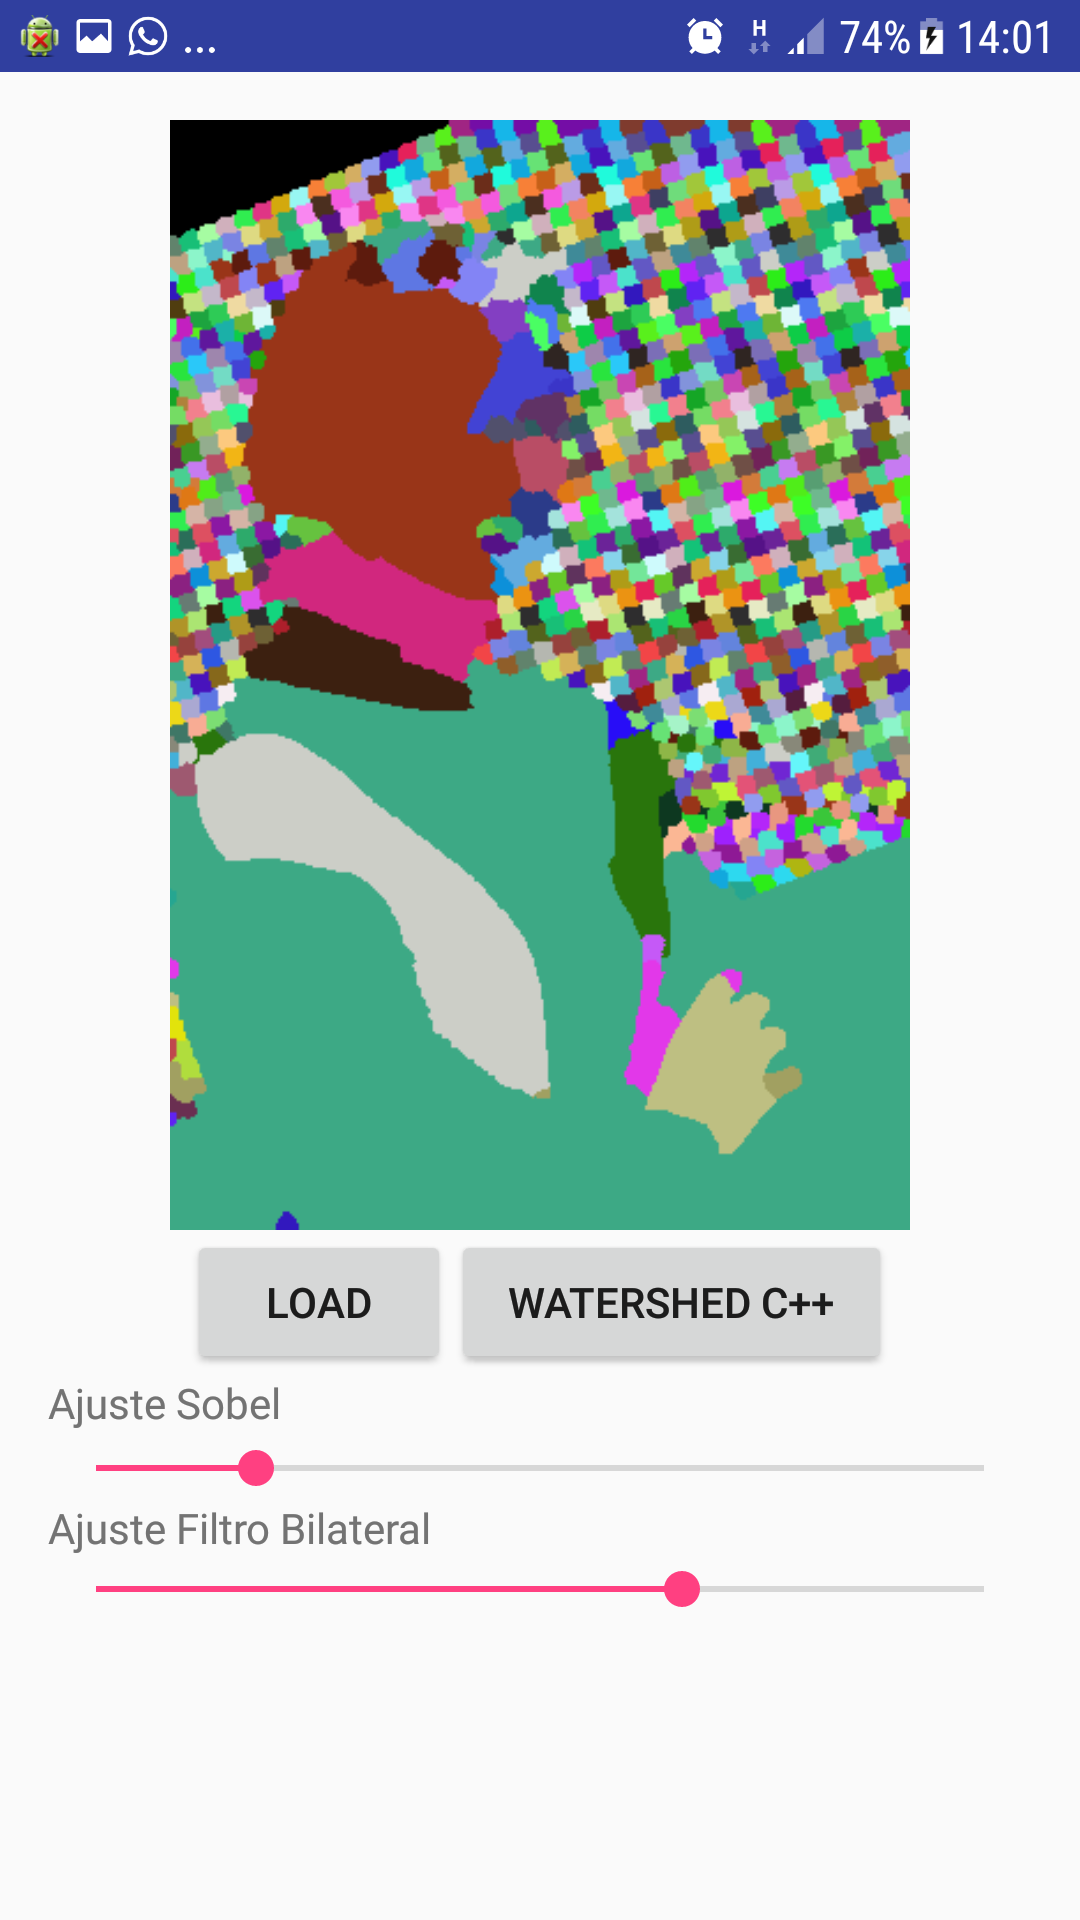
\includegraphics[width=0.4\textwidth]{img/resultado_watershed_desenvolvido_app_n4.png} 
 \caption{\label{fig:resultado_watershed_desenvolvido_app_p4}Resultados de segmentação utilizando o algoritmo \textit{watershed} desenvolvido.}
 %\vspace{2.0em}
\end{figure}
% Figura 
\begin{figure}[!htb]
 \centering
 \def\baselinestretch{1}\small\normalsize
 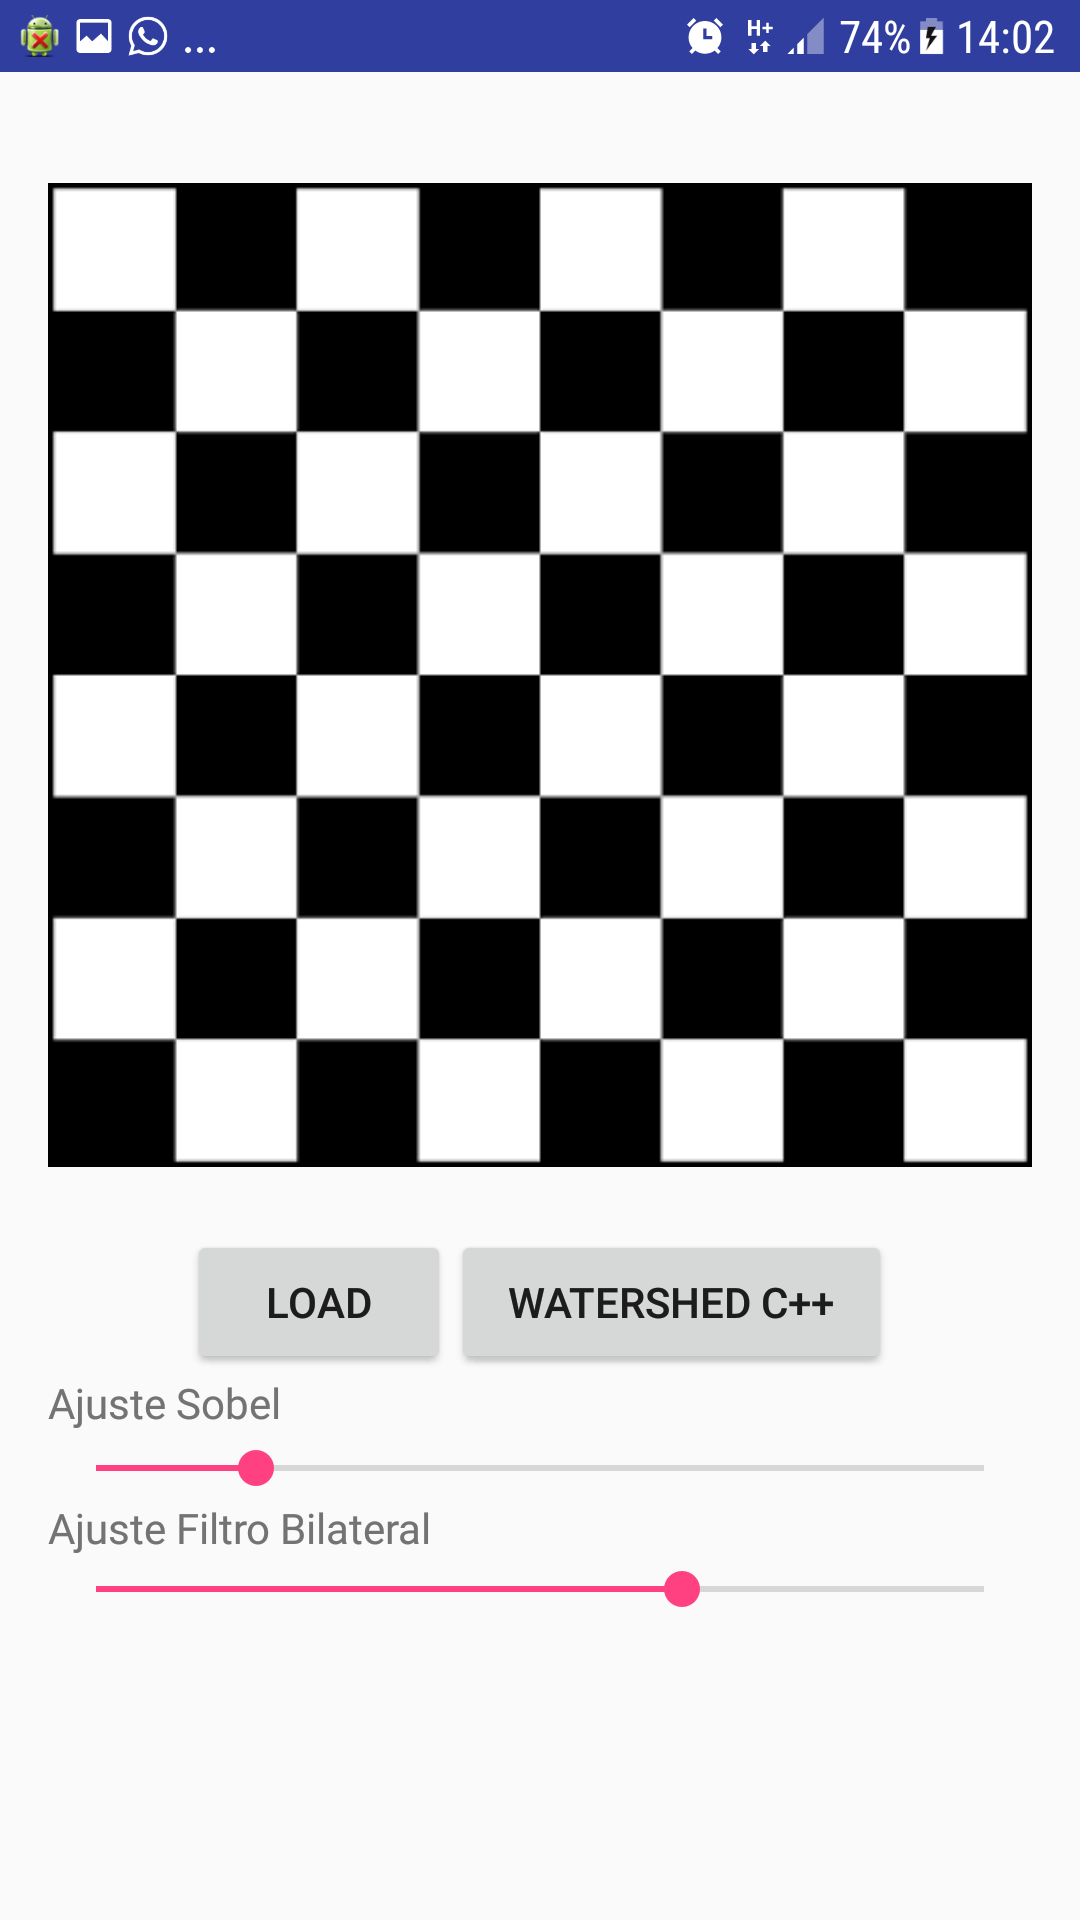
\includegraphics[width=0.4\textwidth]{img/imagem_watershed_desenvolvido_app_n5.png}\qquad
 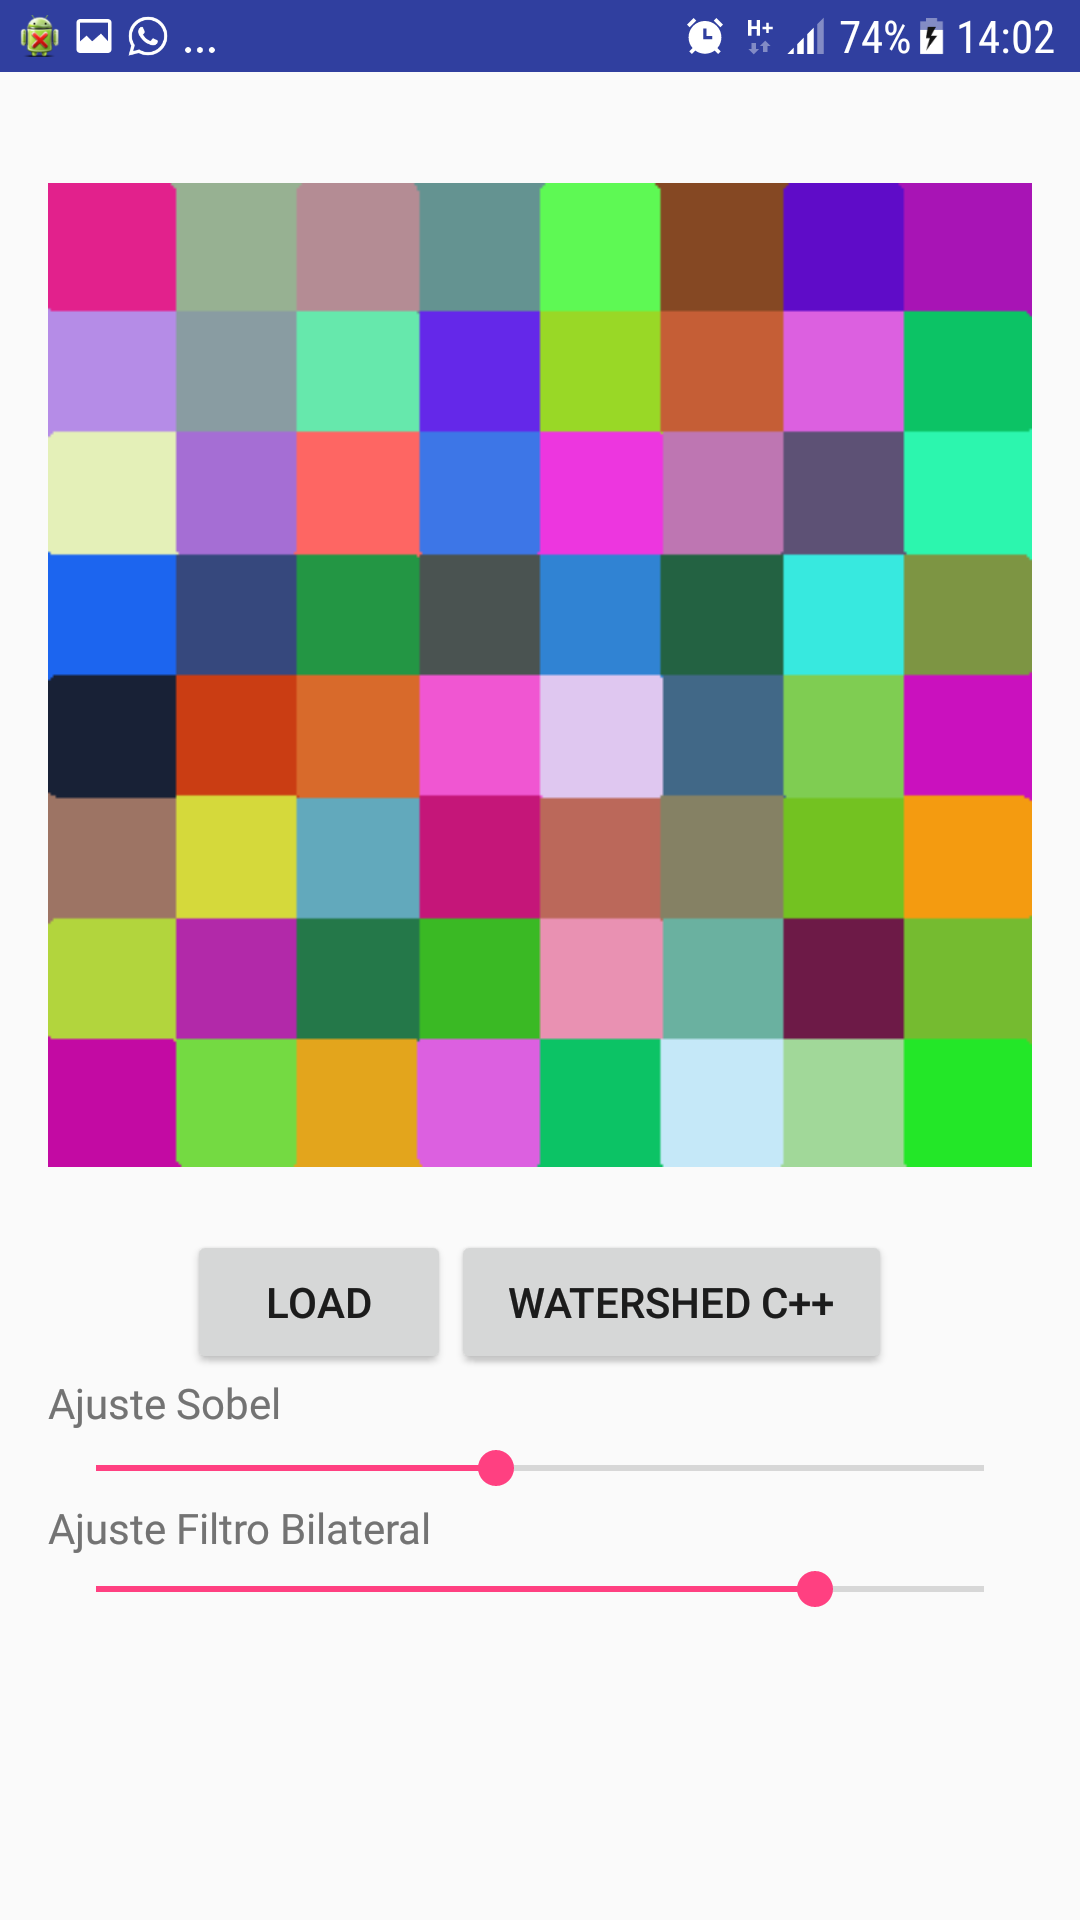
\includegraphics[width=0.4\textwidth]{img/resultado_watershed_desenvolvido_app_n5.png} 
 \caption{\label{fig:resultado_watershed_desenvolvido_app_p5}Resultados de segmentação utilizando o algoritmo \textit{watershed} desenvolvido.}
 %\vspace{2.0em}
\end{figure}
% Figura 
\begin{figure}[!htb]
 \centering
 \def\baselinestretch{1}\small\normalsize
 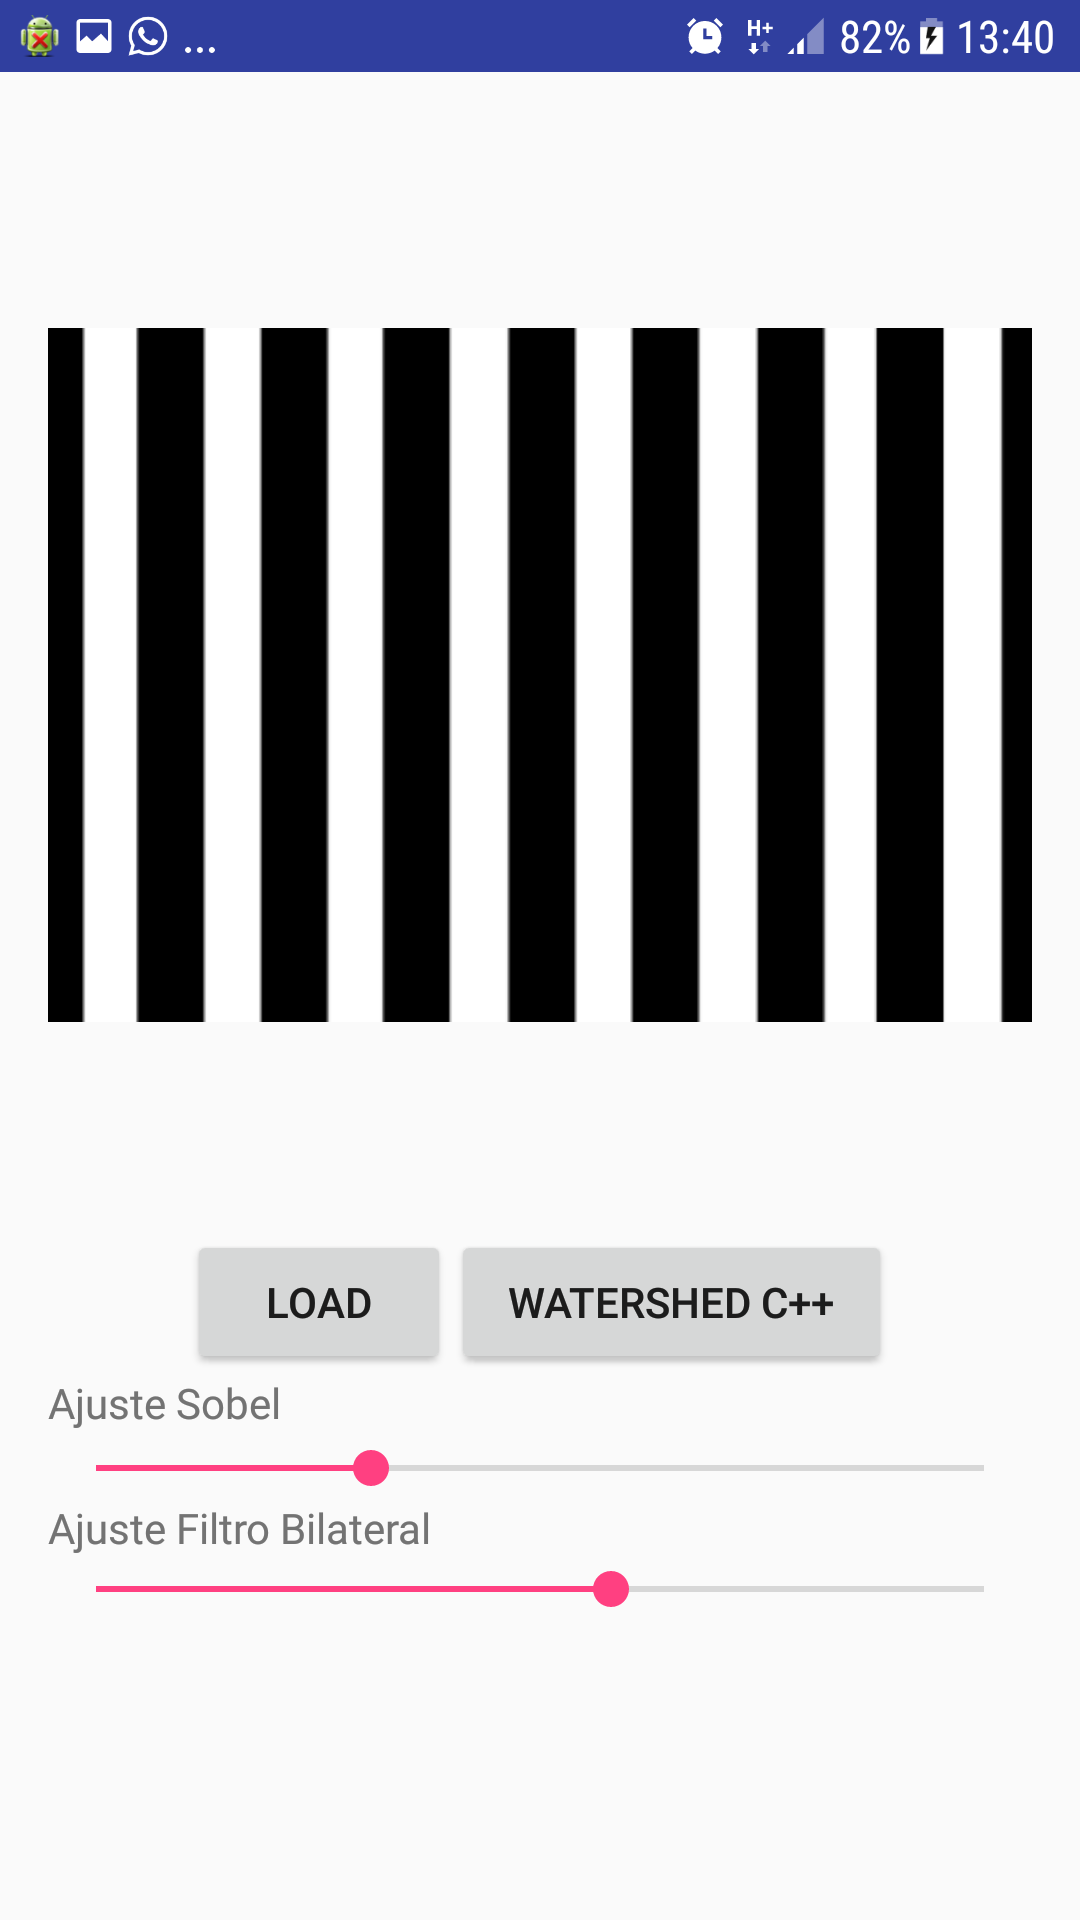
\includegraphics[width=0.4\textwidth]{img/imagem_watershed_desenvolvido_app_n6.png}\qquad
 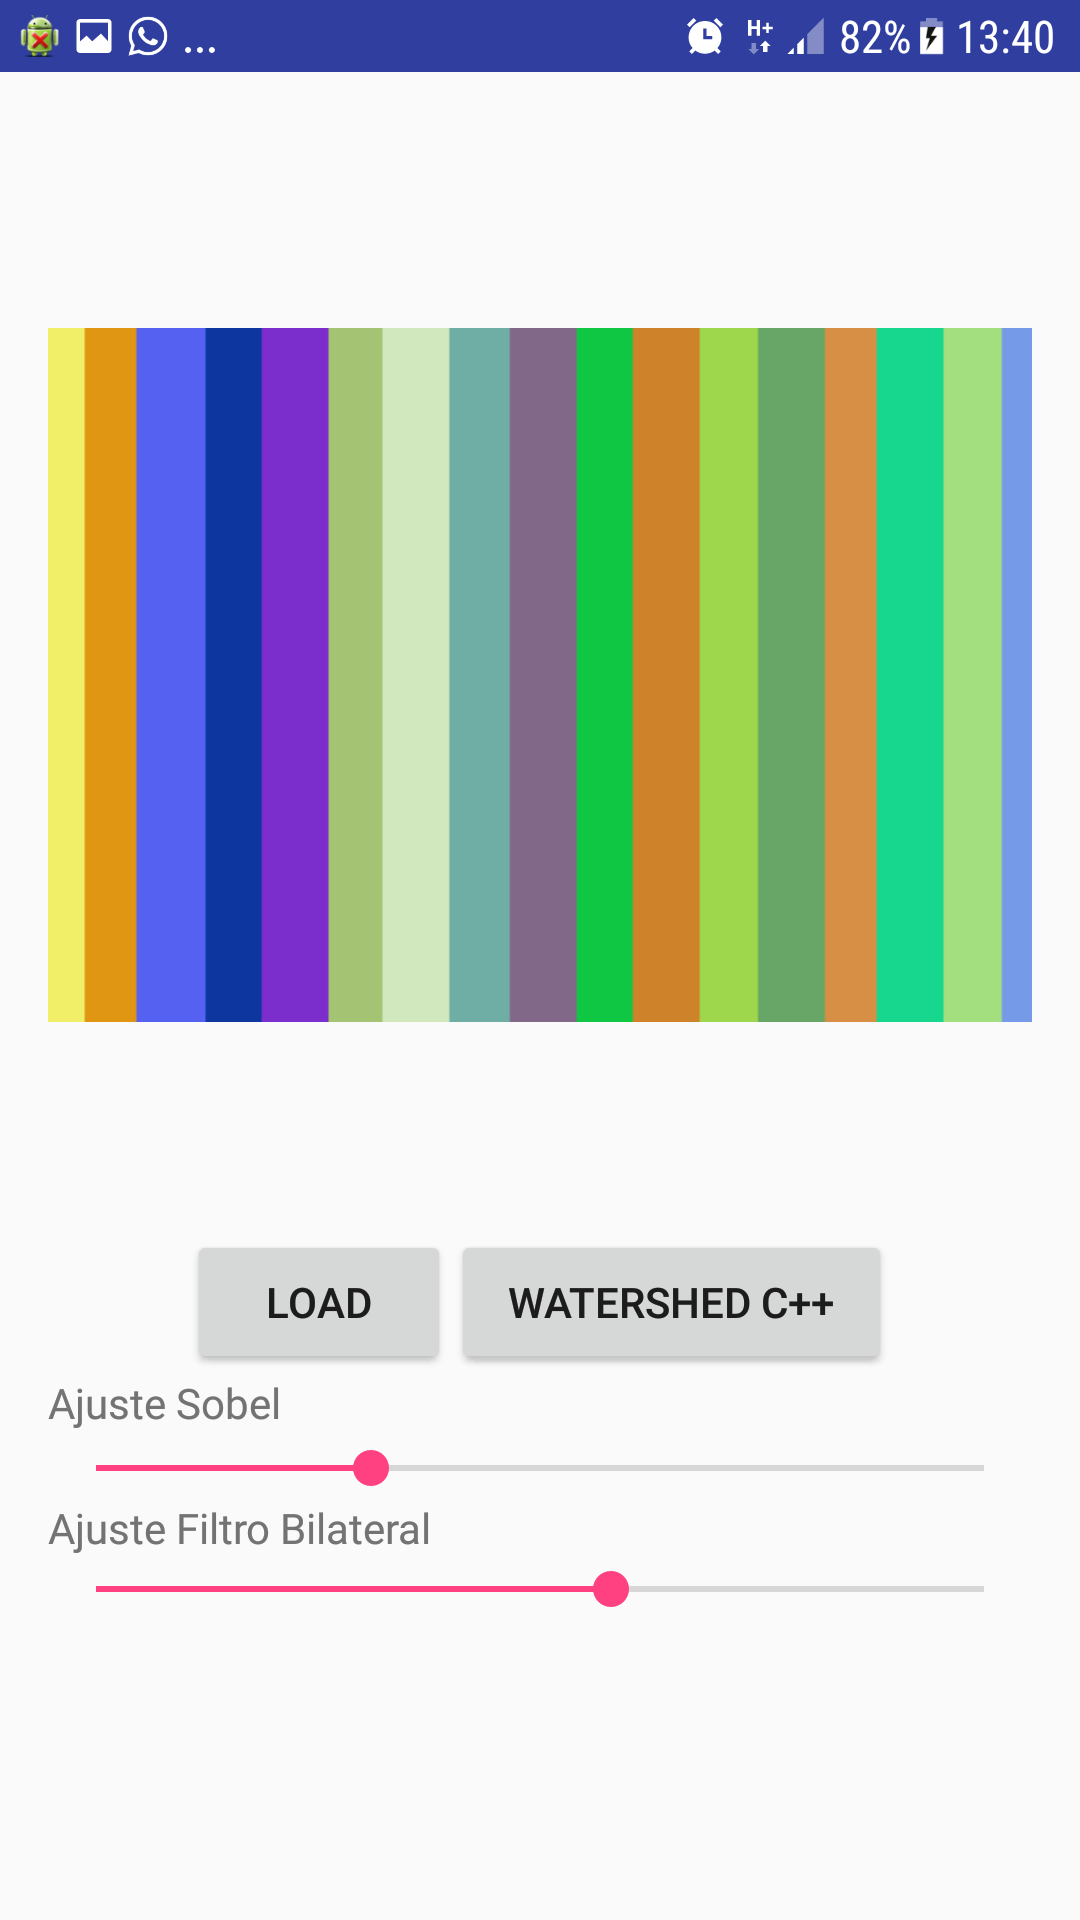
\includegraphics[width=0.4\textwidth]{img/resultado_watershed_desenvolvido_app_n6.png} 
 \caption{\label{fig:resultado_watershed_desenvolvido_app_p6}Resultados de segmentação utilizando o algoritmo \textit{watershed} desenvolvido.}
 %\vspace{2.0em}
\end{figure}
% Figura 
\begin{figure}[!htb]
 \centering
 \def\baselinestretch{1}\small\normalsize
 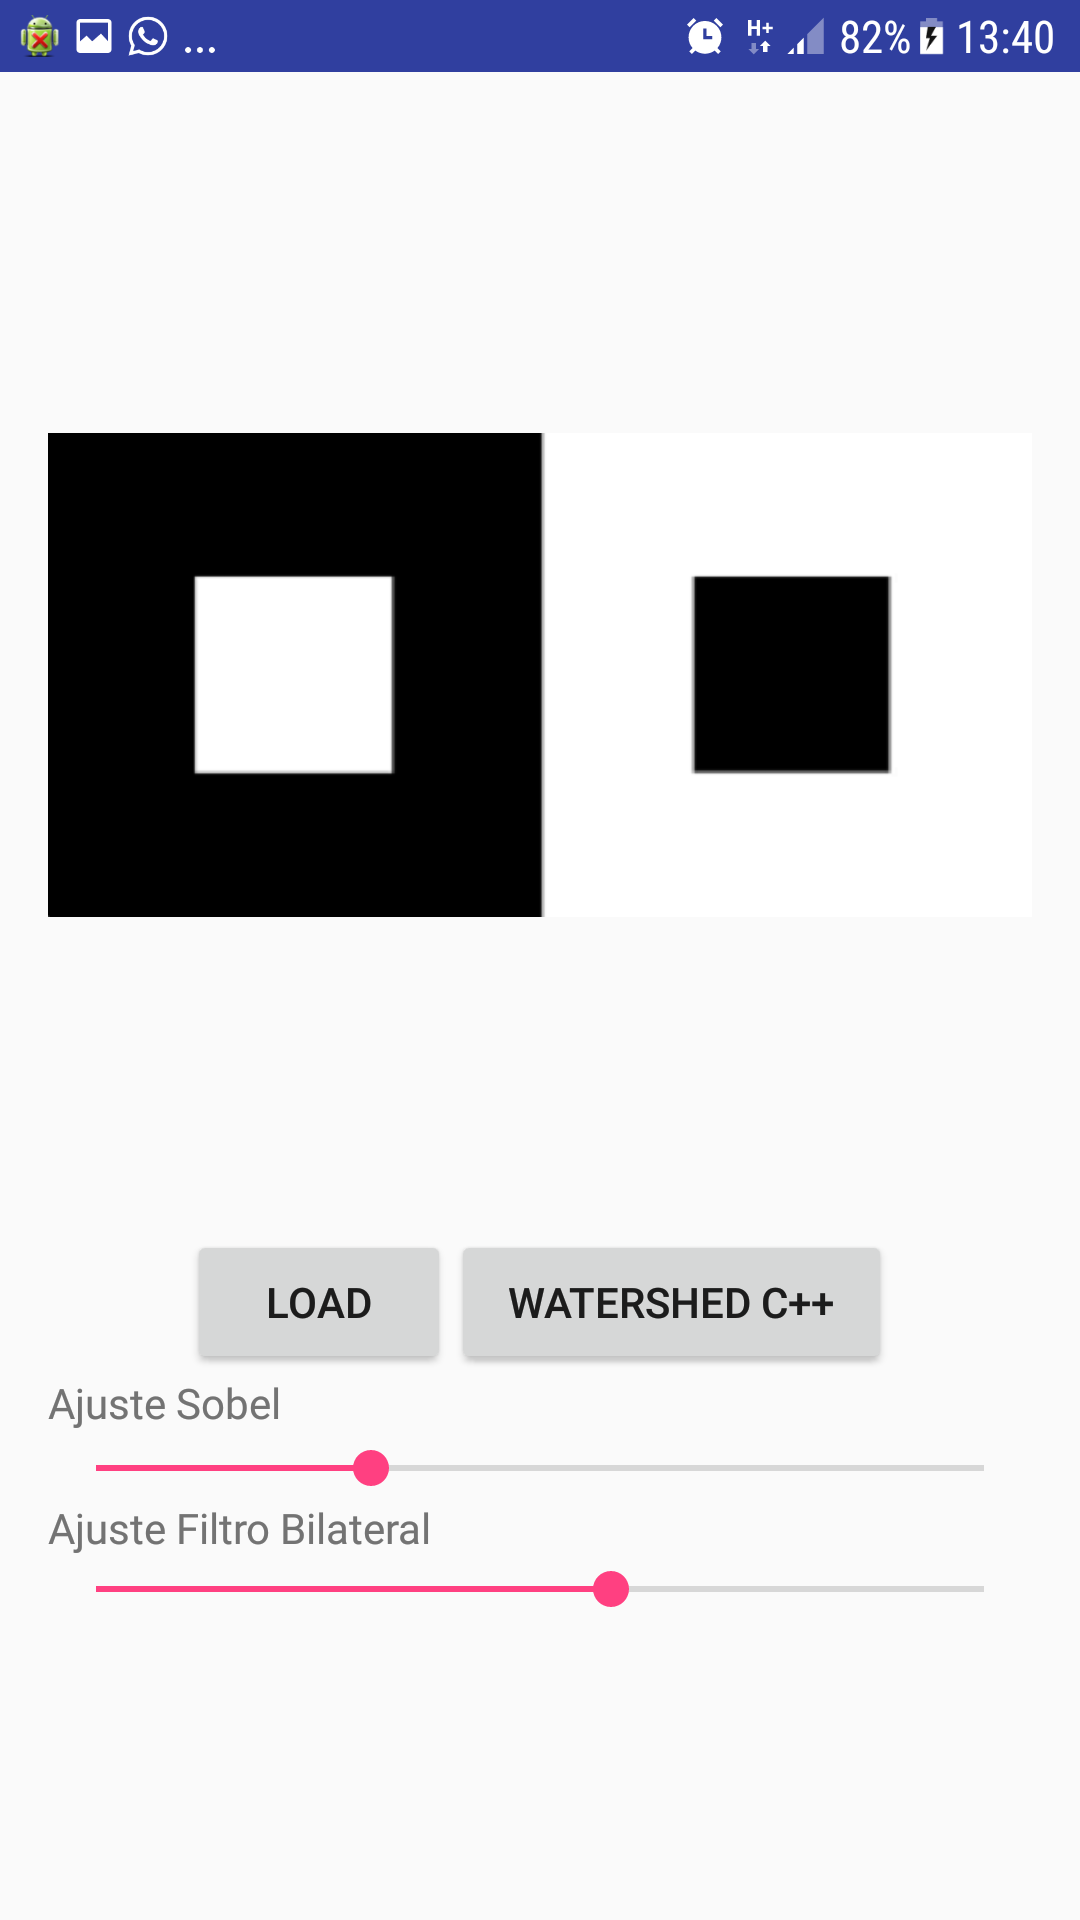
\includegraphics[width=0.4\textwidth]{img/imagem_watershed_desenvolvido_app_n7.png}\qquad
 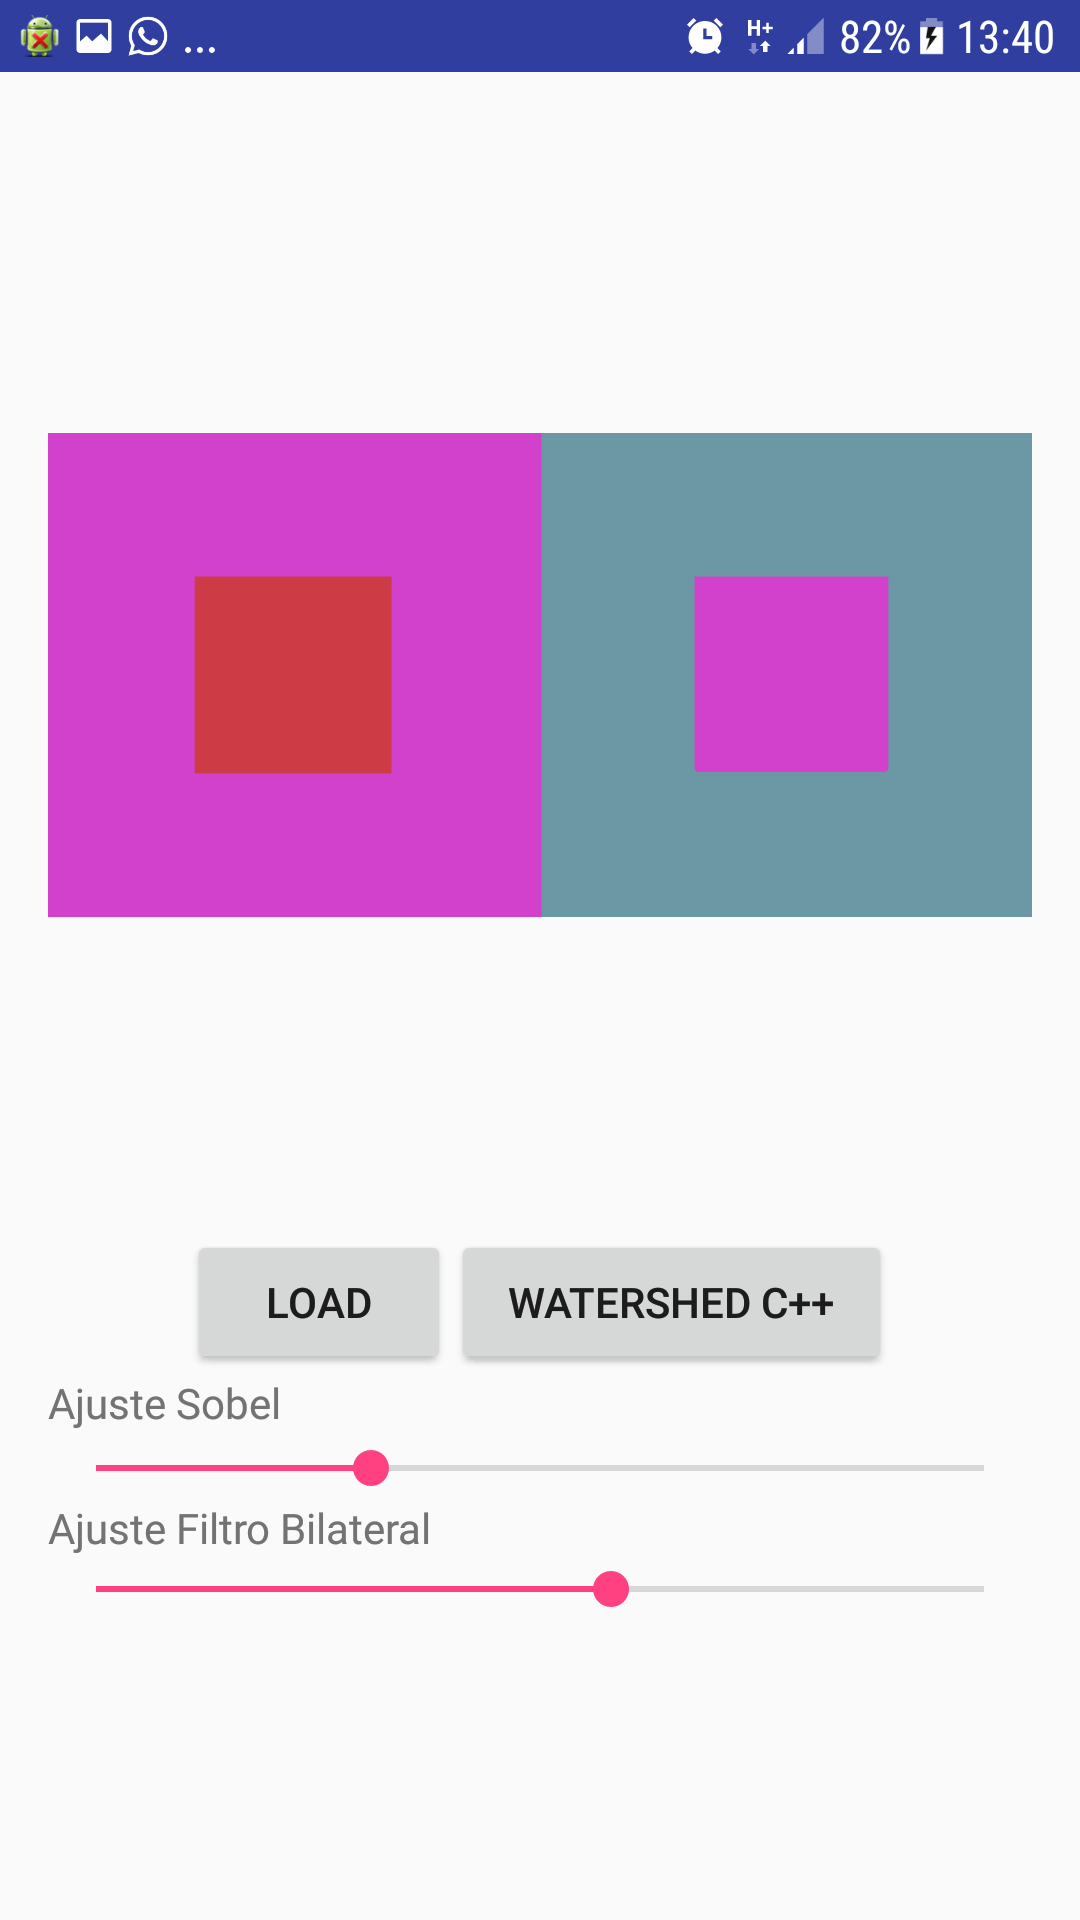
\includegraphics[width=0.4\textwidth]{img/resultado_watershed_desenvolvido_app_n7.png} 
 \caption{\label{fig:resultado_watershed_desenvolvido_app_p7}Resultados de segmentação utilizando o algoritmo \textit{watershed} desenvolvido.}
 %\vspace{2.0em}
\end{figure}	

 

%\subsection{\textit{Watershed} OpenCV Java}

%Da mesma forma, com a imagem escolhida, pode-se optar por segmentá-la através do algoritmo já existente e implementado na interface Java da biblioteca OpenCV. Para isso basta clicar sobre o botão "\textit{watershed} OpenCV" e a imagem resultante da segmentação será apresentada na tela do dispositivo. Enquanto que a imagem resultante pelo processo de segmentação que utiliza o algoritmo desenvolvido para a aplicação é colorida, a imagem resultante da segmentação fornecida pelo OpenCV Java é em níveis de cinza, uma vez que foi assim foi implementada.


%O objetivo de se colocar a segmentação \textit{watershed} fornecida pelo OpenCV Java é possibilitar uma análise comparativa dos resultados obtidos.